\subsection{Implementasi \textit{dashboard}}
komponen \textit{dashboard} dibuat dengan menggunakan bahasa pemrogramman \textit{typescript} dan \textit{vue}. Framework yang digunakan dalam membuat \textit{Dashboard} adalah \textit{Nuxt}. \textit{Nuxt} menjadi pilihan karena memiliki \textit{developer experience} yang bagus serta fitur yang cukup lengkap. \textit{Nuxt} juga memiliki \textit{UI library} yaitu \textit{NuxtUI} yang memudahkan pembuatan \textit{UI}. Pada komponen ini, terdapat 13 halaman yang dapat dikunjungi oleh \textit{user}. Detail dari penjelasan setiap halaman dapat ditemukan pada subbab dibawah ini.

\subsubsection{Halaman \textit{Login}}
Halaman ini berada pada \textit{route} \textbf{/login}. Halaman ini yang berfungsi sebagai \textit{entrypoint} dari komponen \textit{dashboard}. Pada halaman ini terdapat dua input yang di \textit{wrap} oleh sebuah \textit{form}. Input berupa \textit{email} dan \textit{password} \textit{user}. Setelah \textit{user} memasukan \textit{email} dan \textit{password} yang sesuai, maka akan dilakukan \textit{redirect} ke laman utama untuk menunjukan bahwa \textit{user} berhasil terautentikasi dan menggunakan fungsionalitas \textit{dashboard}.

\begin{figure}[h]
  \centering
  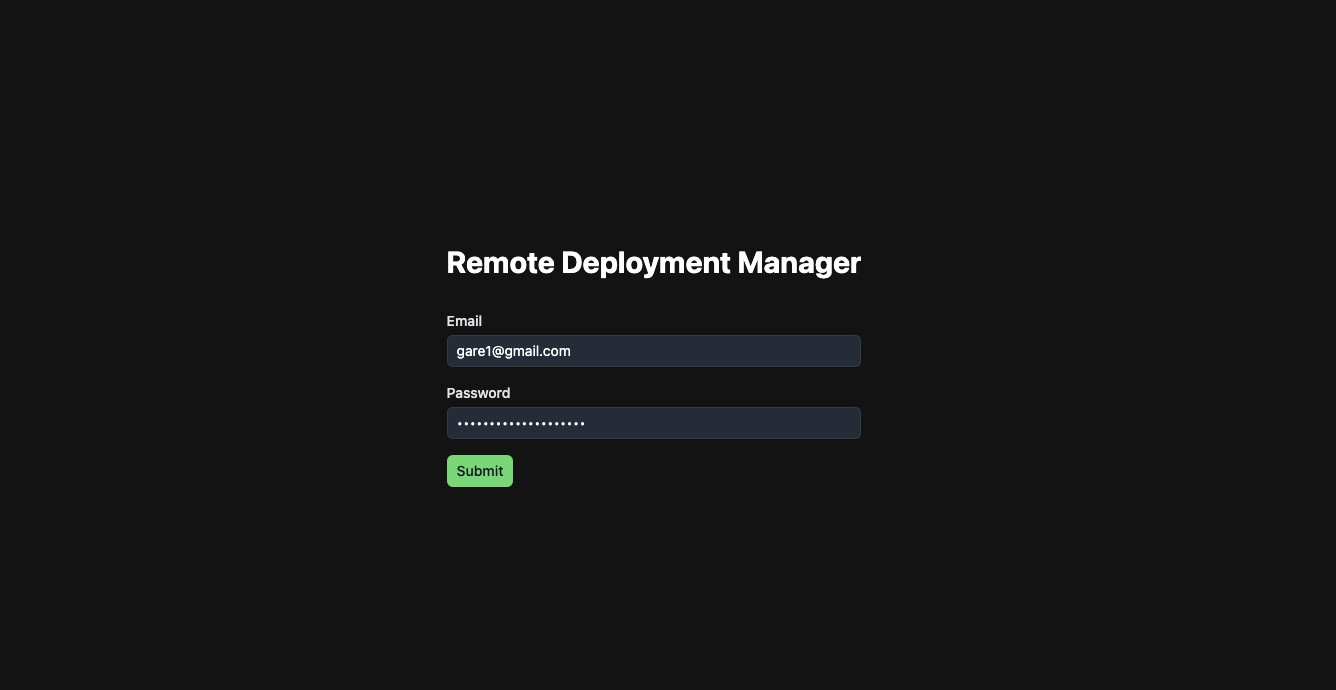
\includegraphics[width=1\textwidth]{resources/chapter-4/dashboard/login-page.jpg}
  \caption{Halaman Login}
  \label{fig:halaman-login}
\end{figure}

\subsubsection{Halaman utama}
Halaman ini merupakan halaman utama dari komponen \textit{dashboard}. Pada halaman ini \textit{user} dapat melihat status dari masing masing objek mulai dari \textit{deployment}, \textit{device}, \textit{group}, serta \textit{quick actions} untuk menuju halaman terkait.

\subsubsection{Halaman \textit{Account}}
Halaman ini berada pada \textit{route \textbf{/account}}. Halaman ini berfungsi untuk memberikan detail mengenai \textit{company} dari \textit{user}. Informasi \textit{company} ditampilkan pada sebuah \textit{card} yang berada pada tengah halaman. Pada halaman ini juga ditampilkan informasi mengenai daftar \textit{user} yang berada pada \textit{company} yang sama dan ditampilkan dengan sebuah tabel. Pada bagian akhir tabel terdapat tombol dengan \textit{icon} elipsis, tombol ini berfungsi sebagai \textit{action} yang dapat dilakukan untuk masing masing \textit{row}

\begin{figure}[h]
  \centering
  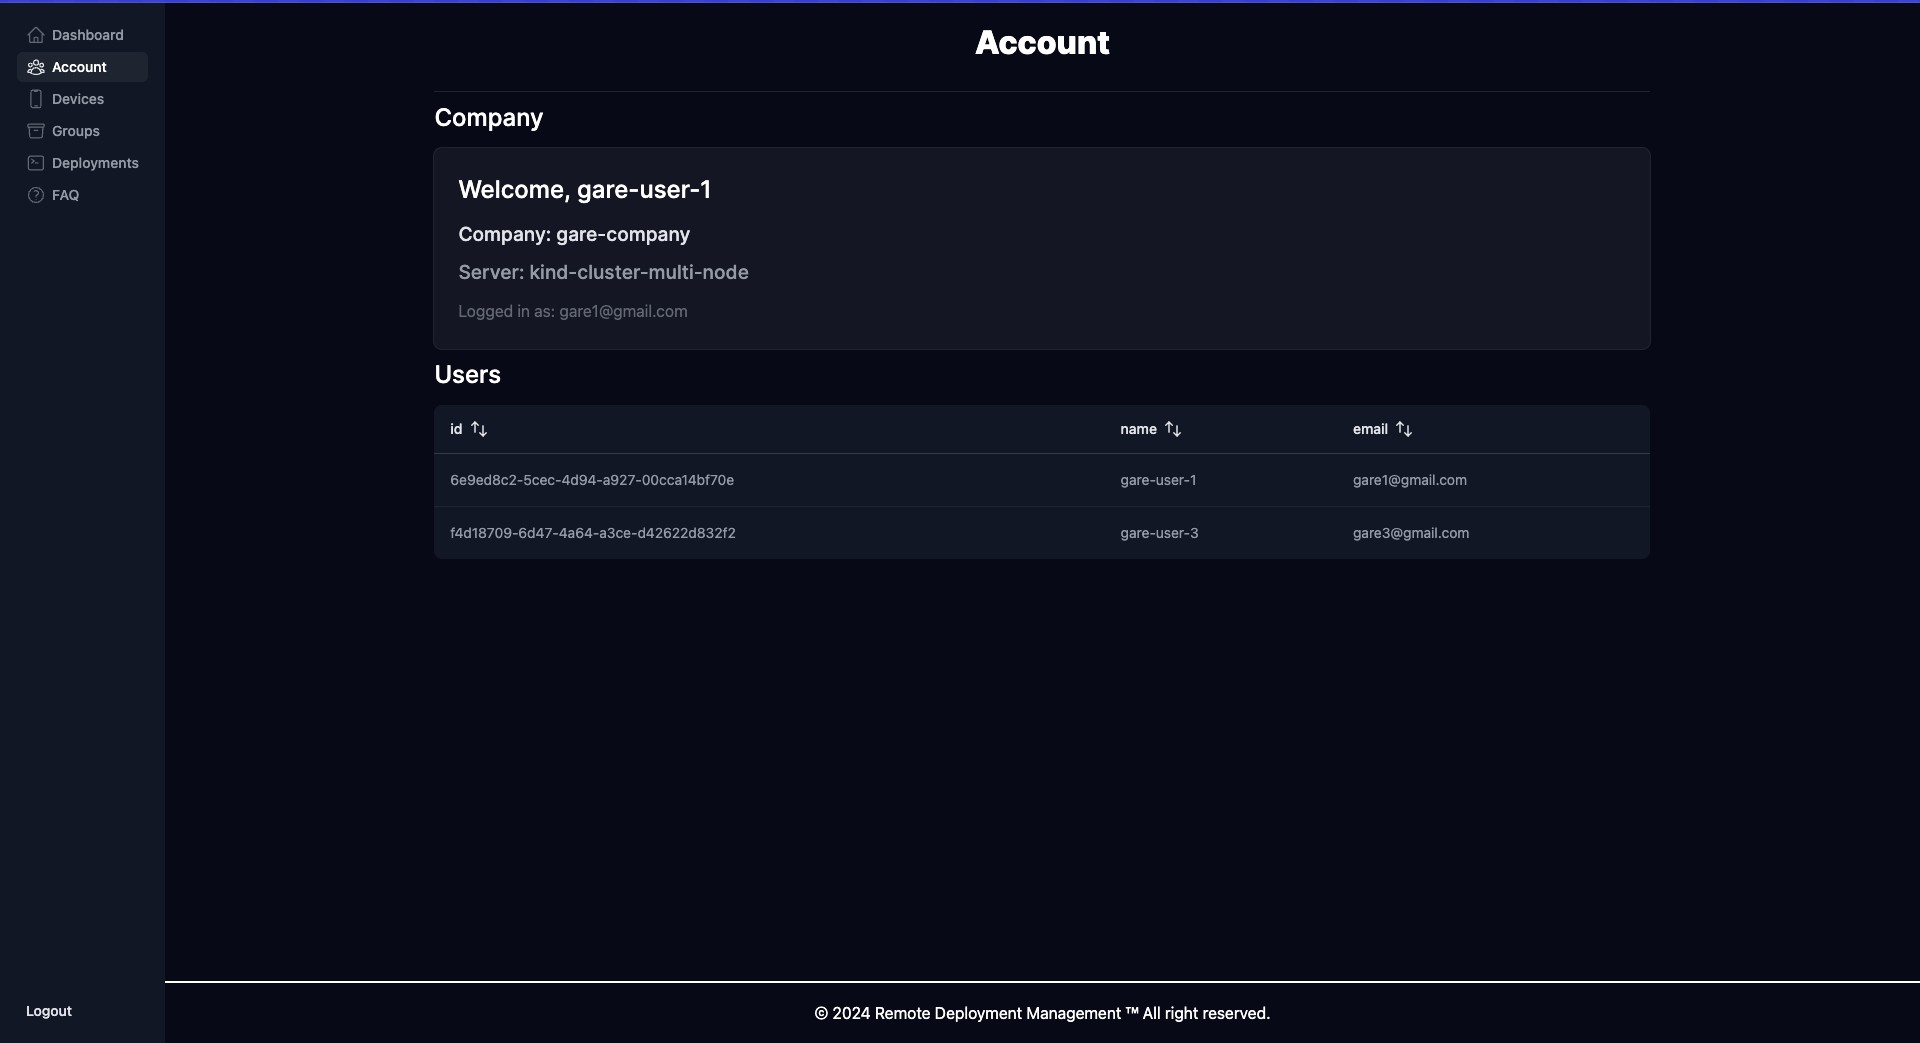
\includegraphics[width=1\textwidth]{resources/chapter-4/dashboard/account-page.jpg}
  \caption{Halaman \textit{account}}
  \label{fig:halaman-account}
\end{figure}

\subsubsection{Halaman \textit{Device}}
Halaman ini berada pada \textit{route \textbf{/devices}}. Halaman ini berfungsi untuk melakukan manajemen \textit{device} pada satu perusahaan. Halaman ini menunjukan informasi seluruh \textit{device} yang terdaftar pada \textit{company}.

\begin{figure}[h]
  \centering
  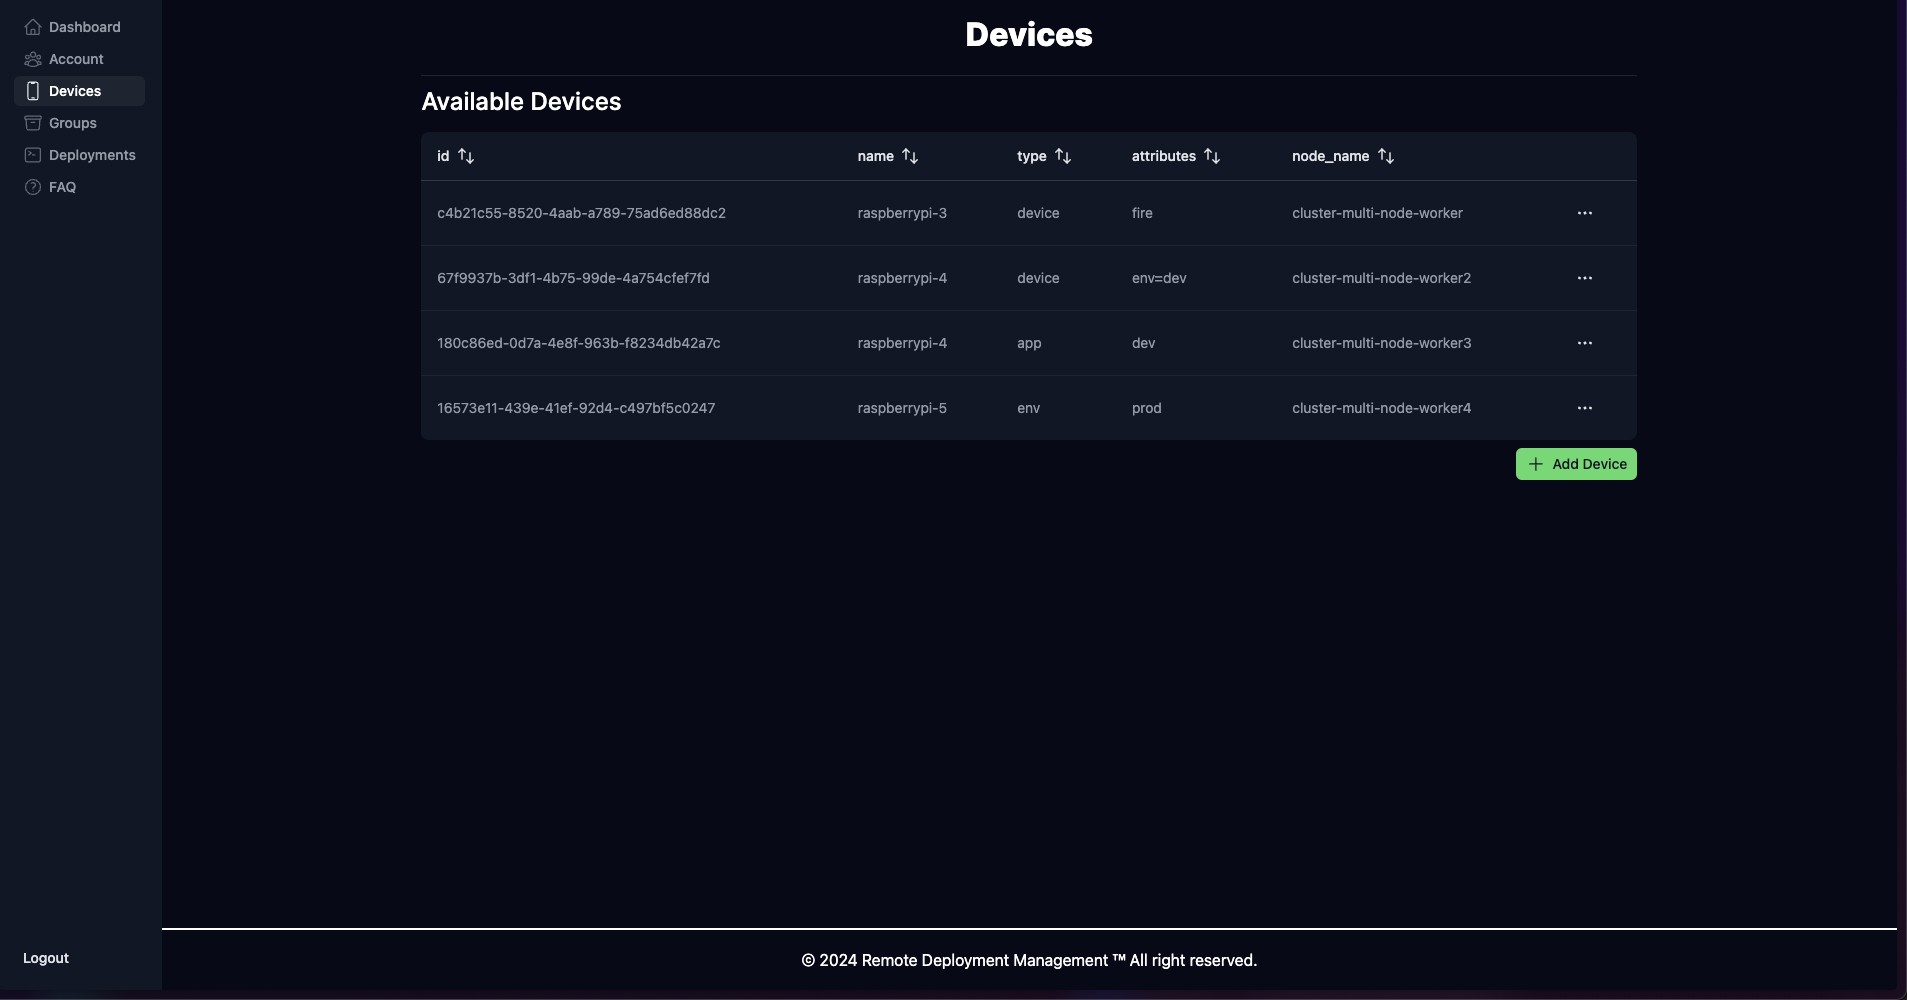
\includegraphics[width=1\textwidth]{resources/chapter-4/dashboard/device-page.jpg}
  \caption{Halaman \textit{device}}
  \label{fig:halaman-device}
\end{figure}

Sama seperti halaman \textit{account}, terdapat tombol dengan icon elipsis pada bagian kanan untuk melakukan fungsi seperti melihat detail ataupun menghapus \textit{device} terkait. Apabila \textit{user} menekan tombol \textit{detail} maka user akan diarahkan ke halaman \textbf{/device/:id} sesuai dengan id \textit{device} yang dipilih

\begin{figure}[h]
  \centering
  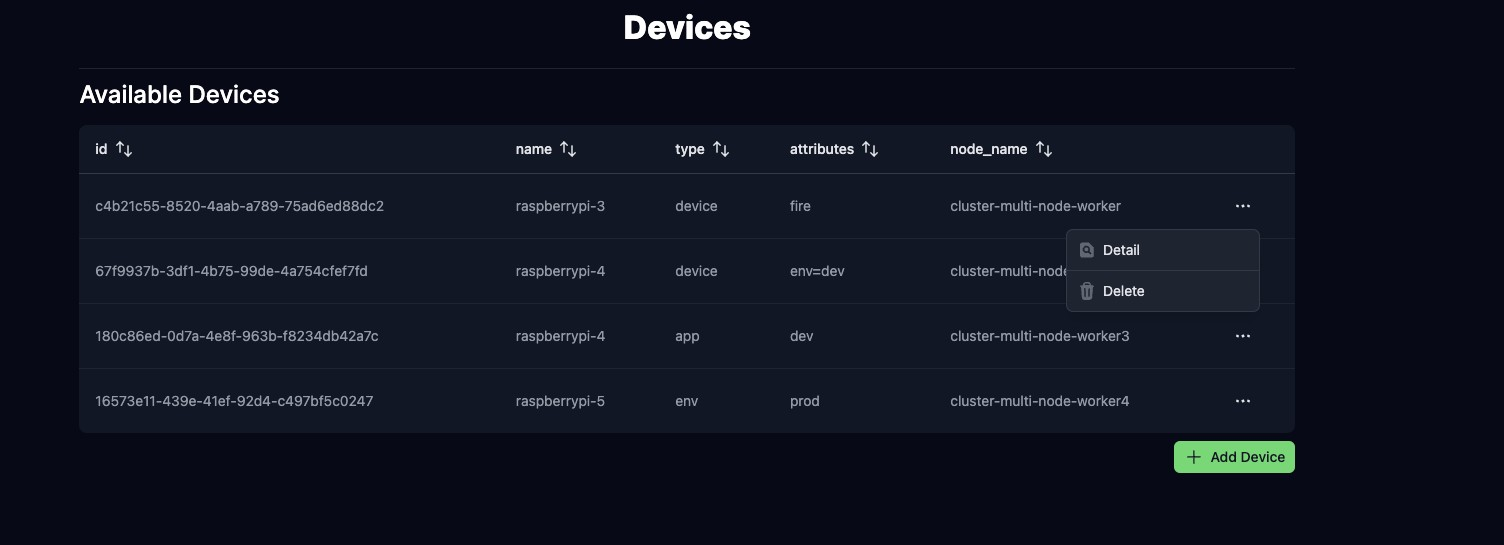
\includegraphics[width=1\textwidth]{resources/chapter-4/dashboard/device-page-actions.jpg}
  \caption{Actions pada table \textit{device}}
  \label{fig:halaman-device-actions}
\end{figure}

Pada halaman ini terdapat tombol yang dapat ditekan untuk menambahkan \textit{device}. Apabila ditekan akan muncul sebuah modal. Modal ini berisi input yang dapat \textit{user} isi untuk membuat sebuah \textit{device} baru pada sistem. Terdapat validasi pada setiap input, setelah semua validasi dilewati maka barulah tombol \textit{submit} akan mengirimkan \textit{request} ke \textit{server} untuk di proses.

Akan muncul sebuah notifikasi pada bagian kanan bawah tergantung \textit{response} yang diberikan oleh \textit{server}. Warna hijau menandakan bahwa \textit{response} sukses dan warna \textit{merah} menandakan bahwa terdapat masalah ketika memproses \textit{request}.

\begin{figure}[h]
  \centering
  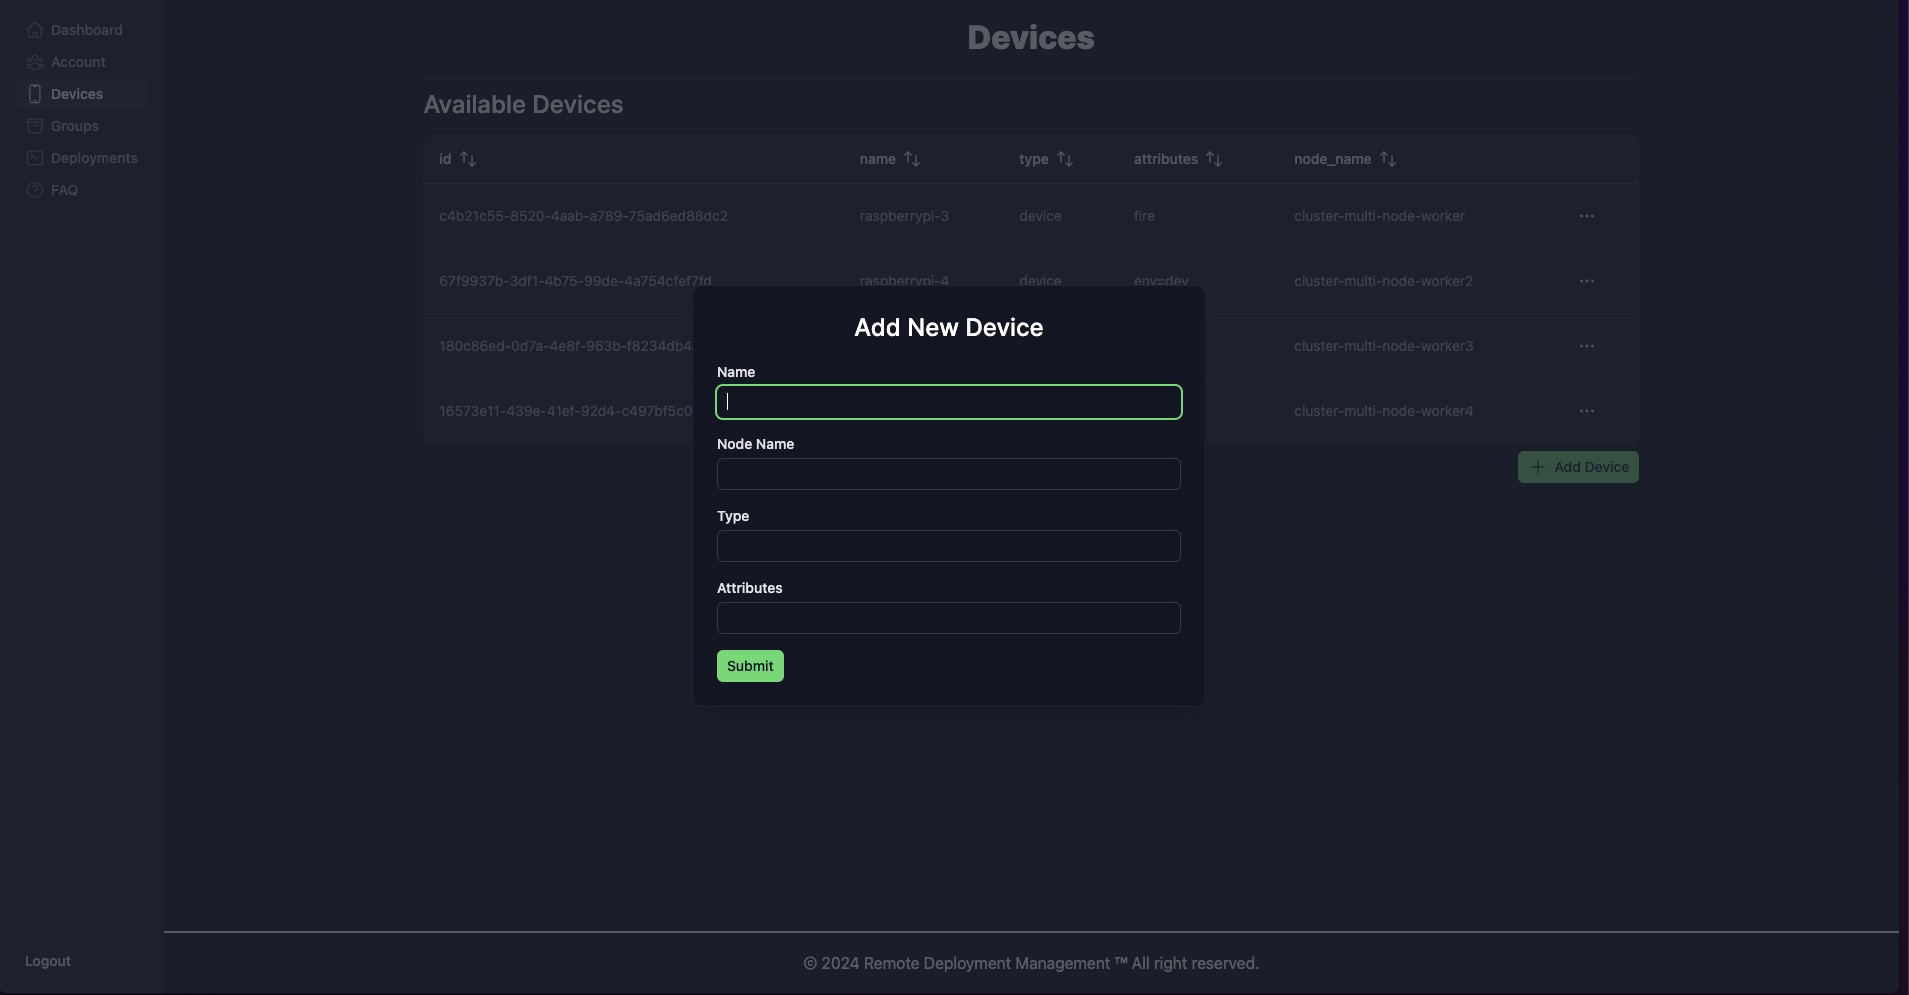
\includegraphics[width=1\textwidth]{resources/chapter-4/dashboard/device-page-add.jpg}
  \caption{Modal menambahkan \textit{device}}
  \label{fig:halaman-device-add}
\end{figure}



\pagebreak

\subsubsection{Halaman \textit{Device detail}}
penjelasan halaman device detail
\begin{figure}[h]
  \centering
  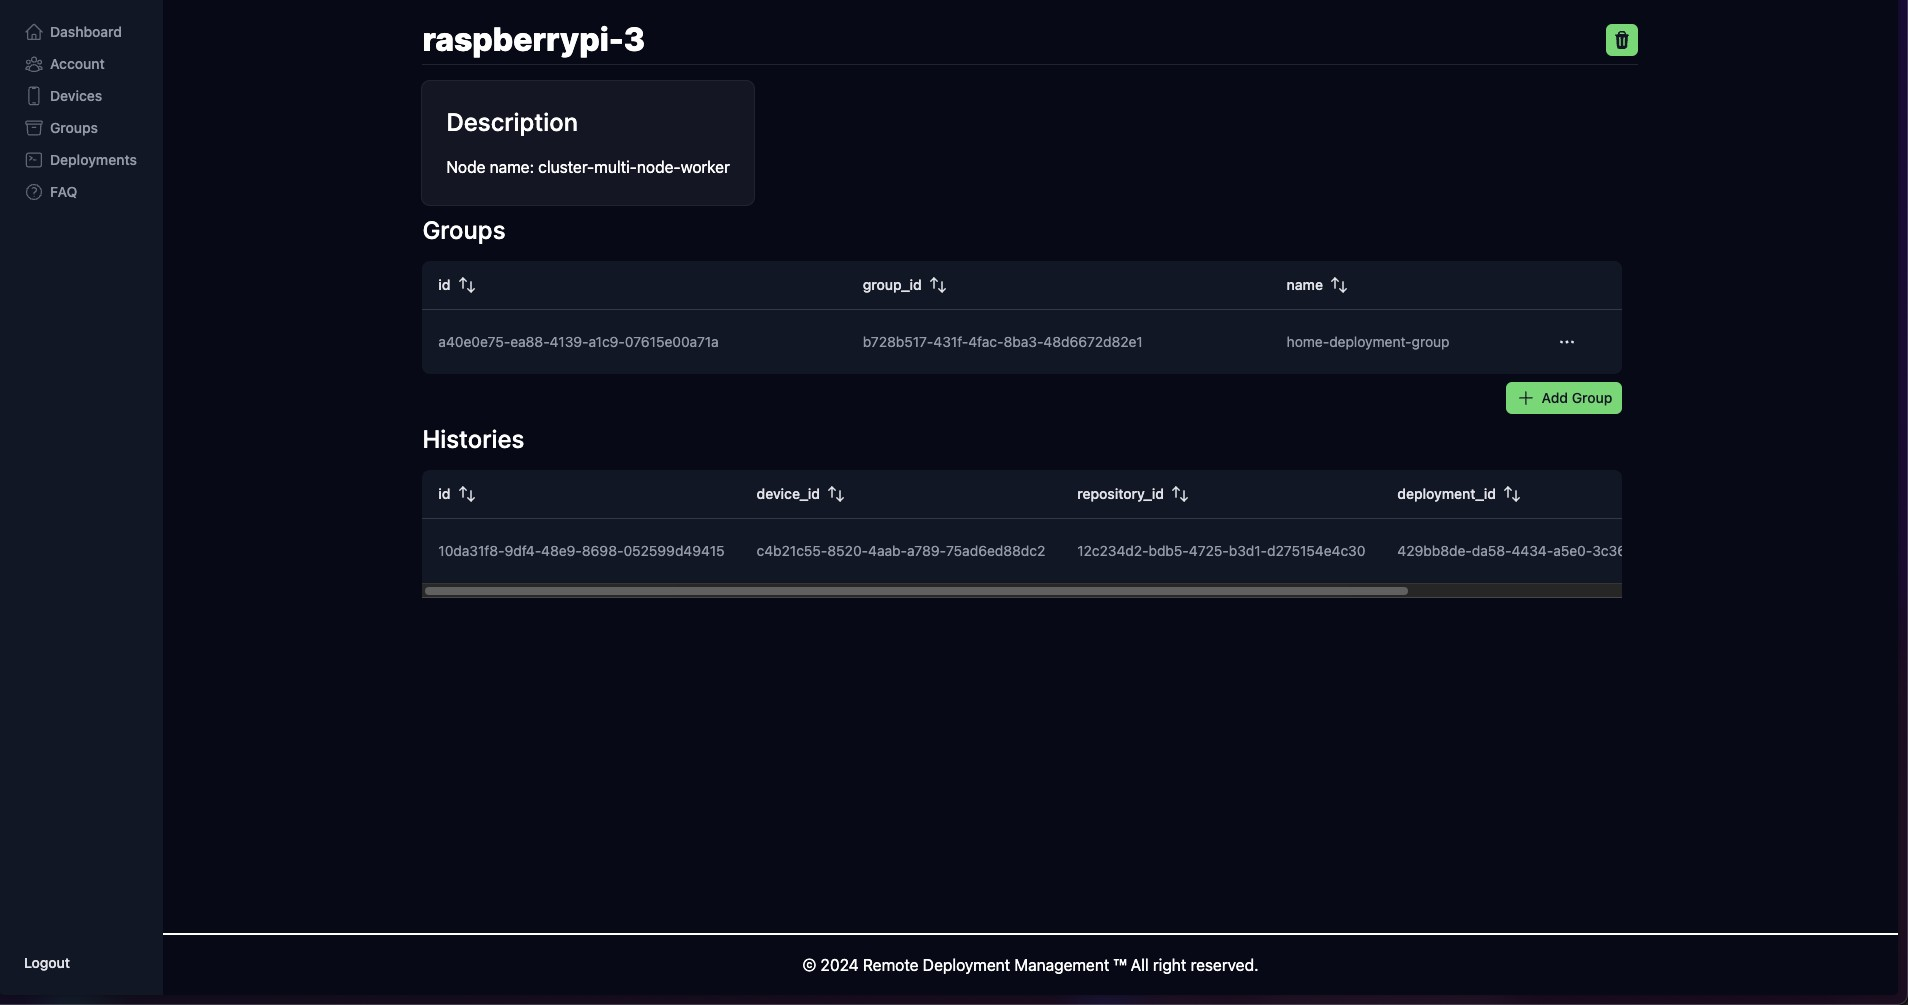
\includegraphics[width=1\textwidth]{resources/chapter-4/dashboard/device-detail-page.jpg}
  \caption{Halaman \textit{device detail}}
  \label{fig:halaman-device-detail}
\end{figure}

\begin{figure}[h]
  \centering
  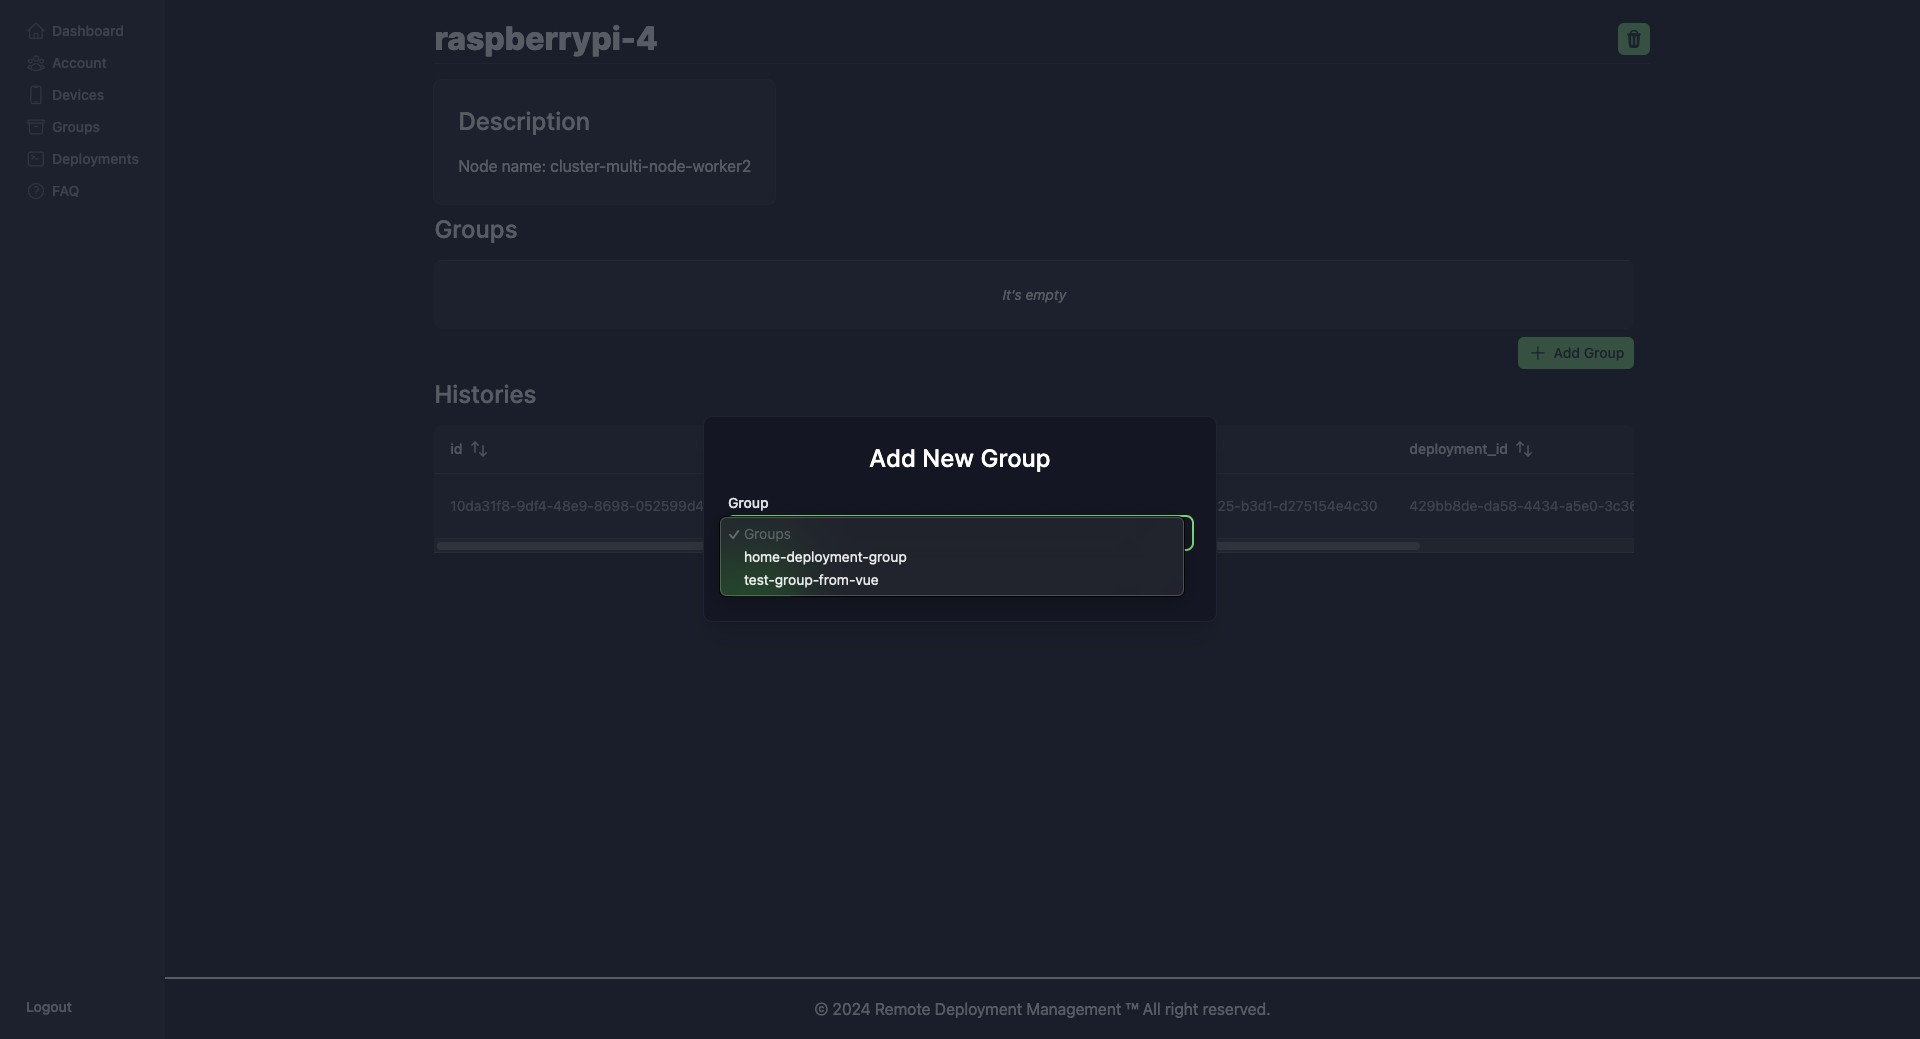
\includegraphics[width=1\textwidth]{resources/chapter-4/dashboard/device-detail-add-group.jpg}
  \caption{Modal menambahkan group pada \textit{device detail}}
  \label{fig:halaman-device-detail-add-group}
\end{figure}

\begin{figure}[h]
  \centering
  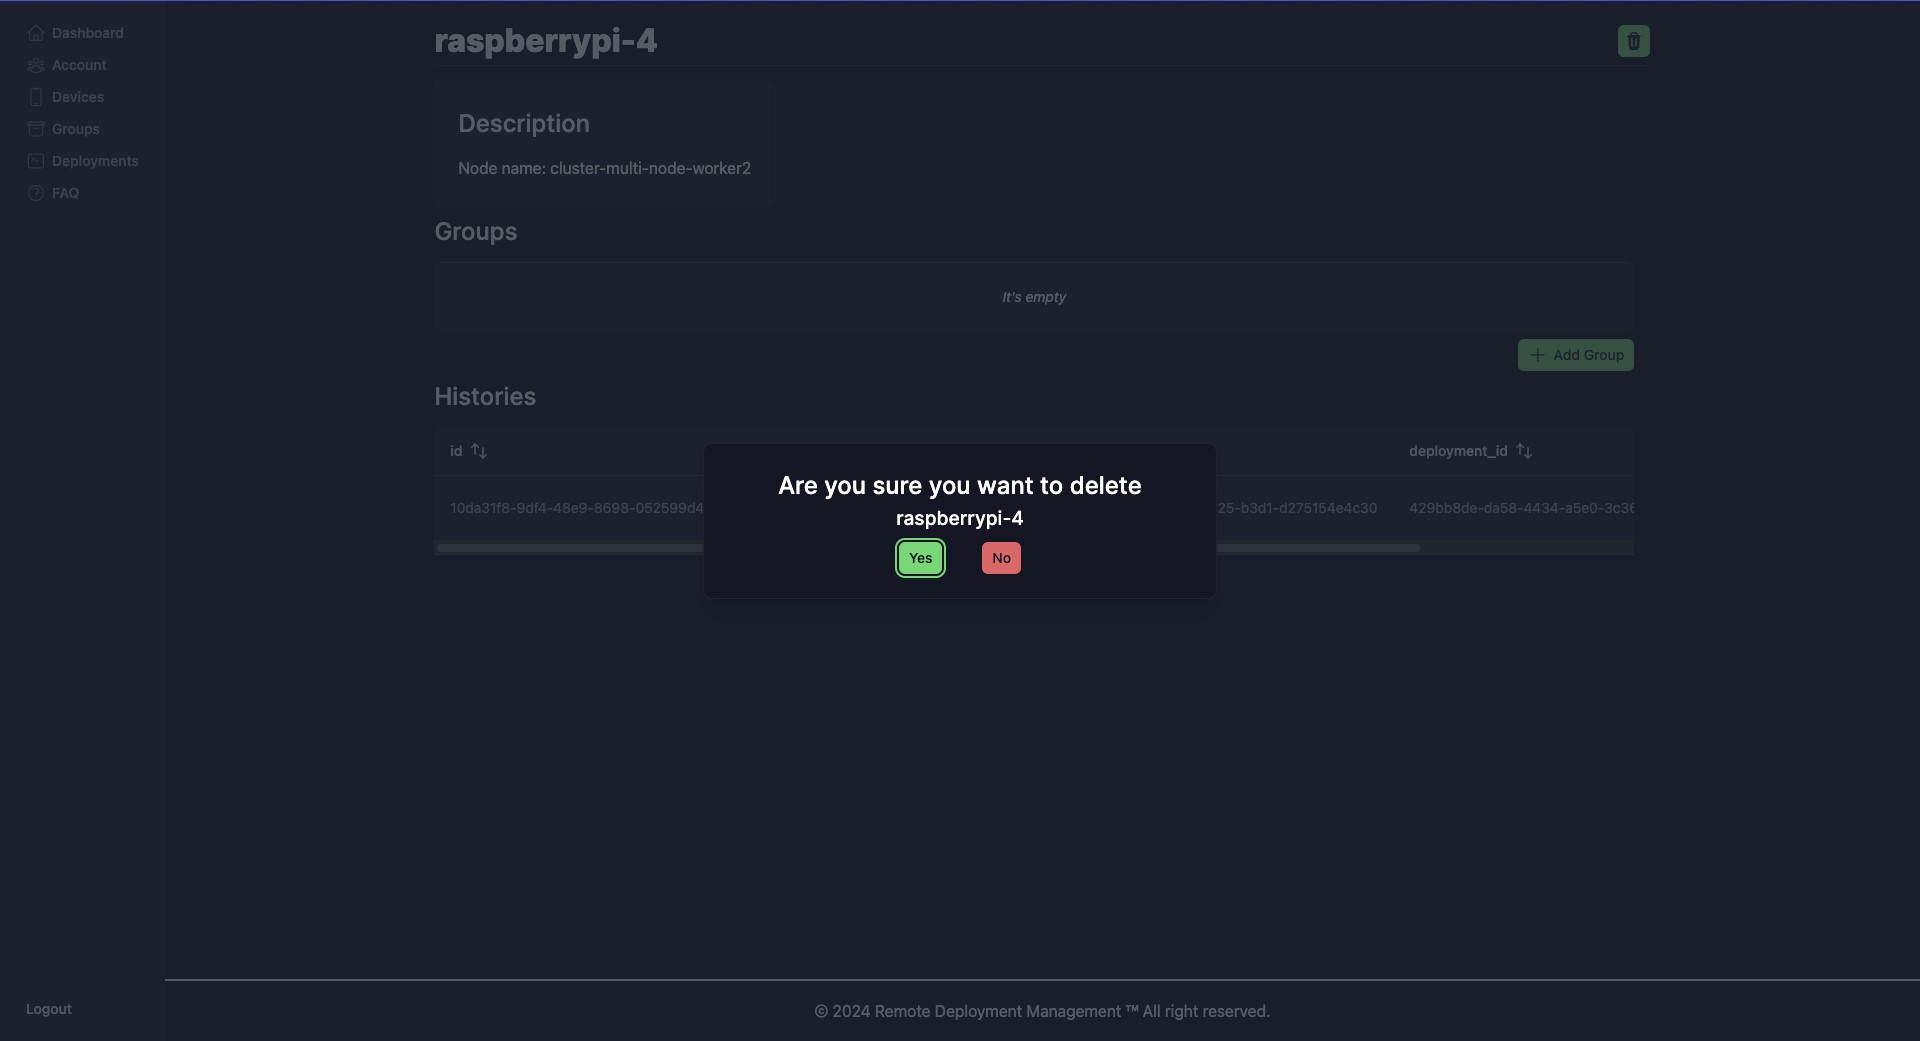
\includegraphics[width=1\textwidth]{resources/chapter-4/dashboard/device-detail-delete.jpg}
  \caption{Modal menghapus device pada halaman \textit{device detail}}
  \label{fig:halaman-device-detail-delete}
\end{figure}

\pagebreak

\subsubsection{Halaman \textit{Groups}}
penjelasan halaman groups
\begin{figure}[h]
  \centering
  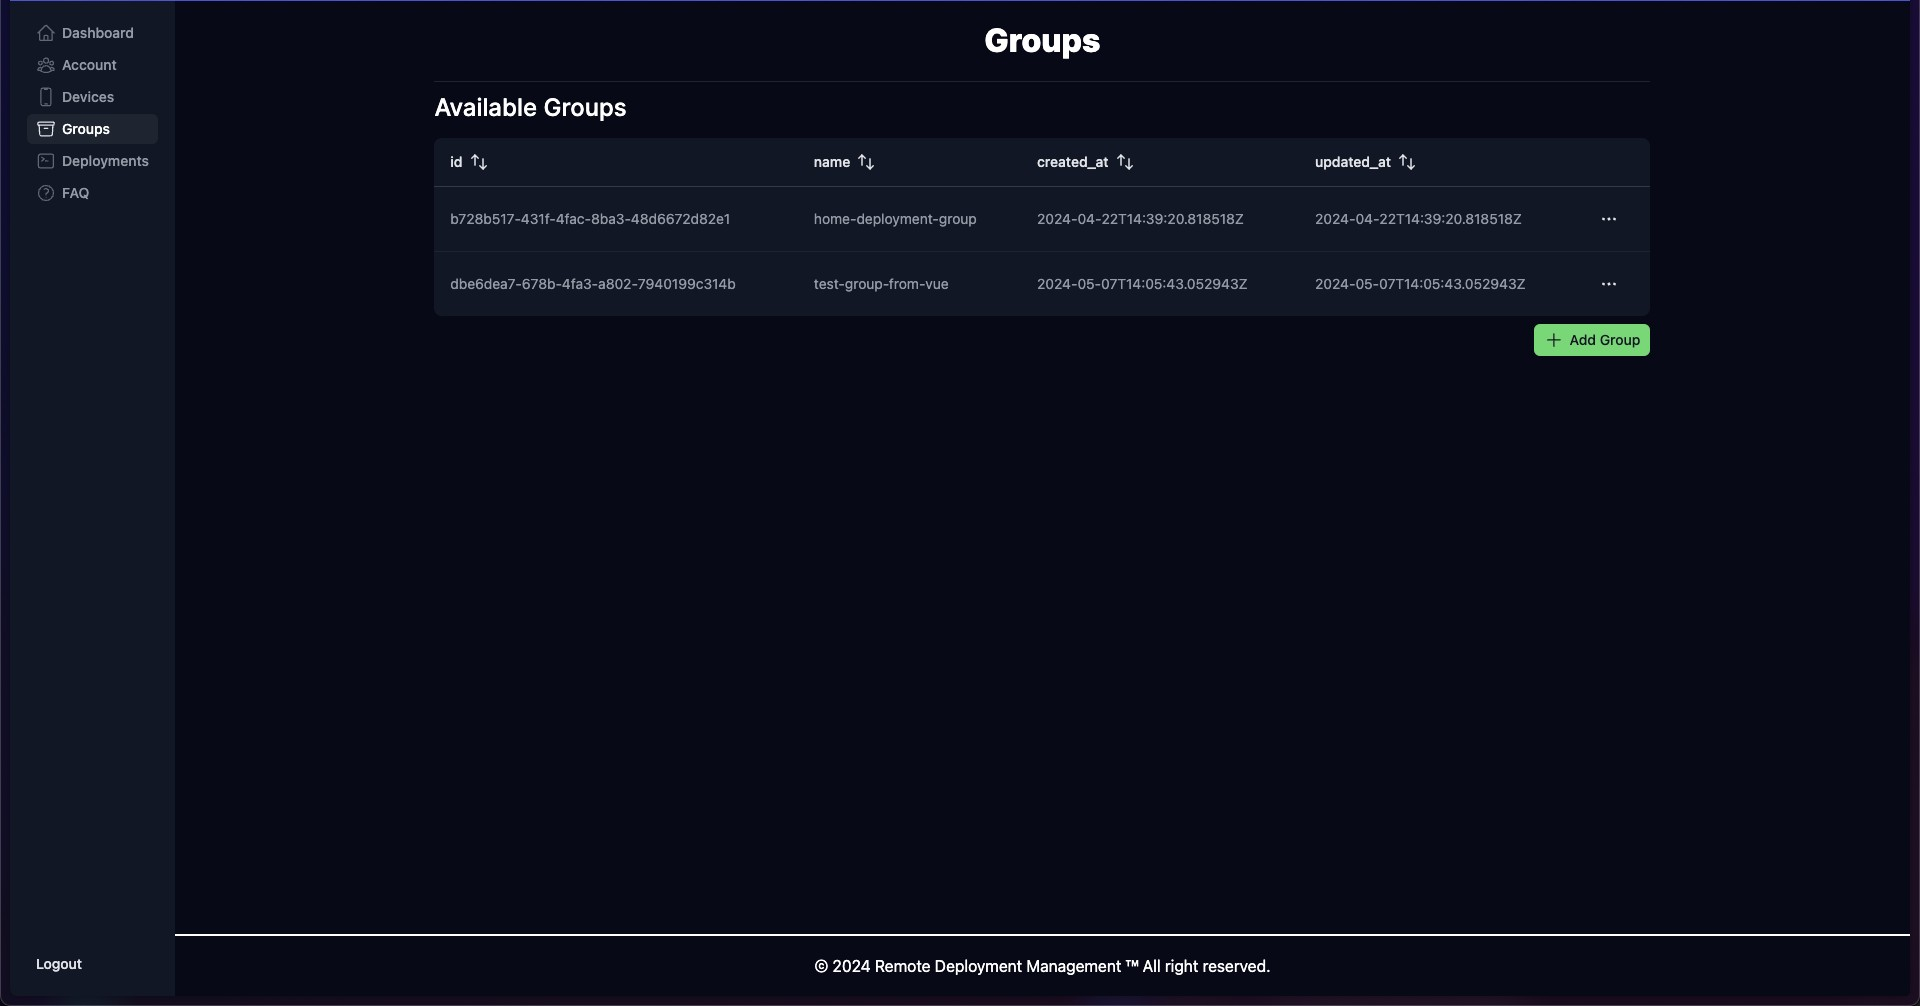
\includegraphics[width=1\textwidth]{resources/chapter-4/dashboard/groups-page.jpg}
  \caption{Halaman \textit{groups}}
  \label{fig:halaman-groups}
\end{figure}

\begin{figure}[h]
  \centering
  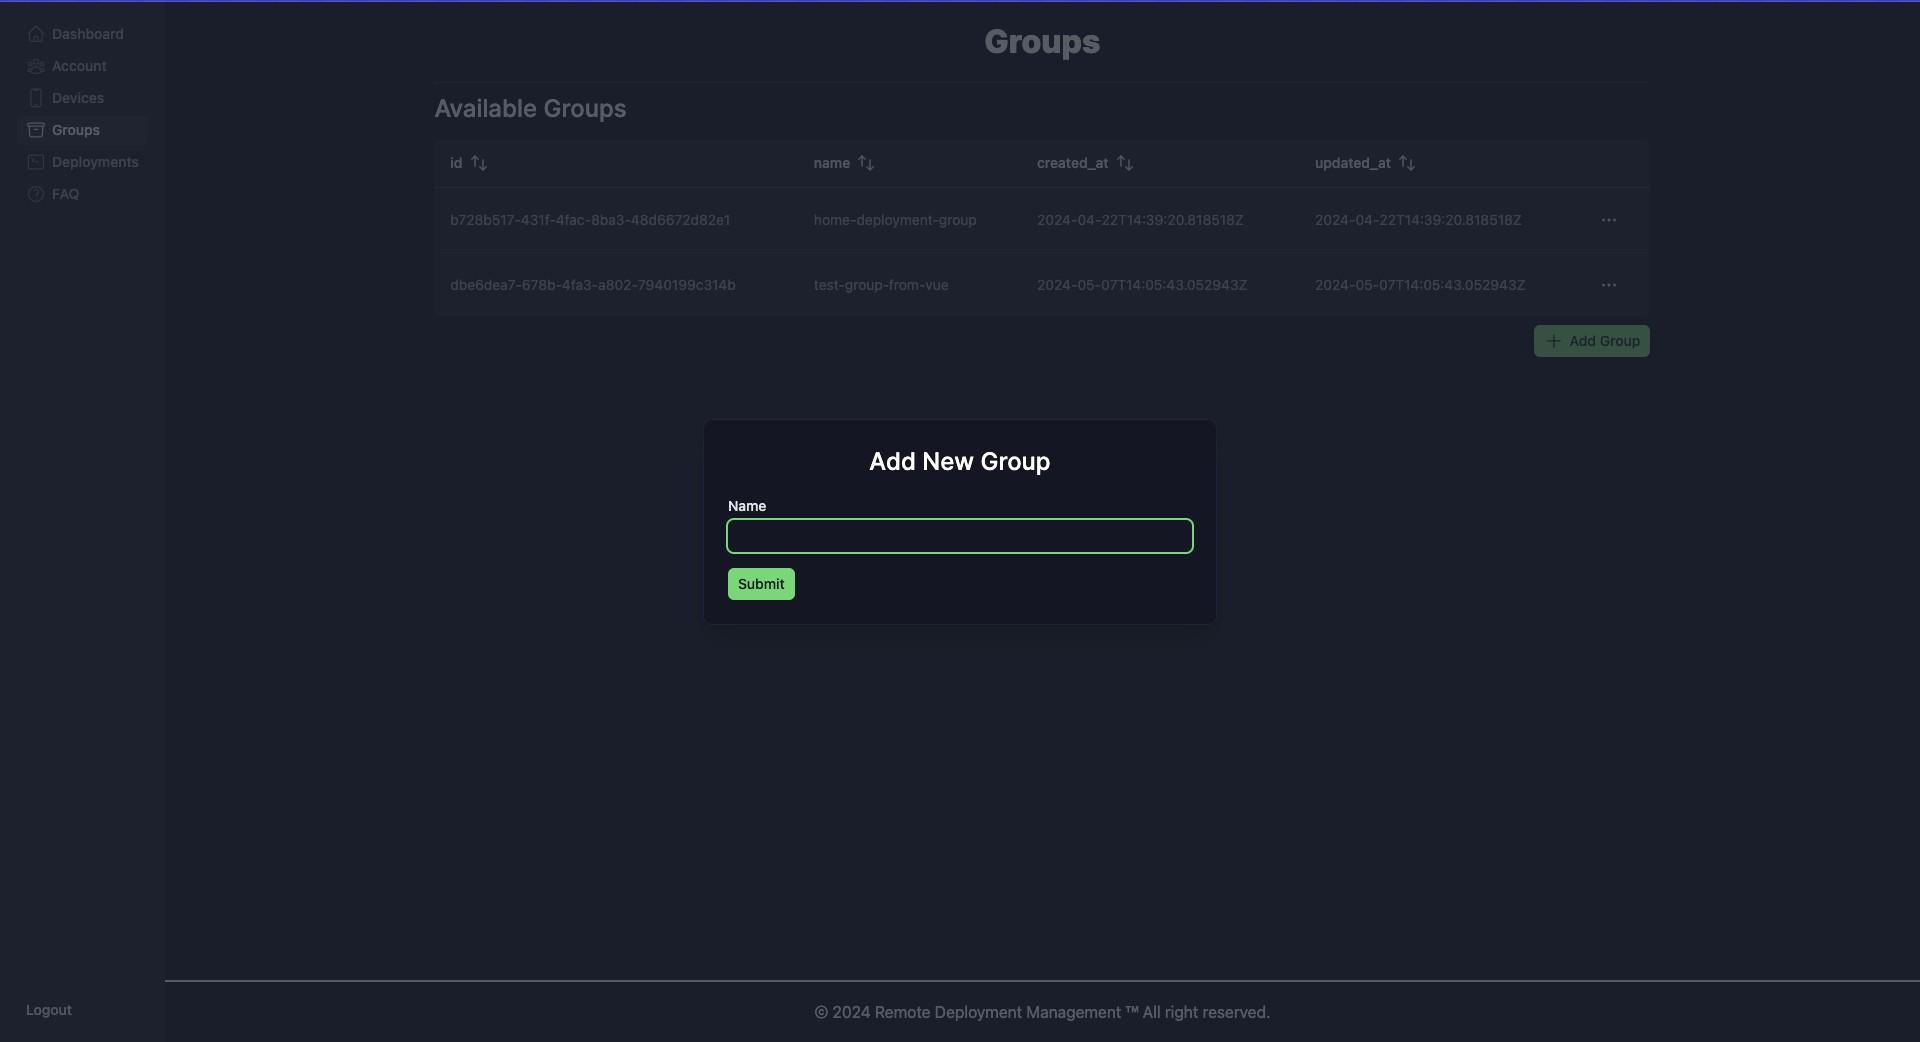
\includegraphics[width=1\textwidth]{resources/chapter-4/dashboard/groups-page-add.jpg}
  \caption{Modal menambahkan \textit{groups}}
  \label{fig:halaman-groups-add}
\end{figure}

\pagebreak

\subsubsection{Halaman \textit{Groups detail}}
penjelasan halaman groups detail
\begin{figure}[h]
  \centering
  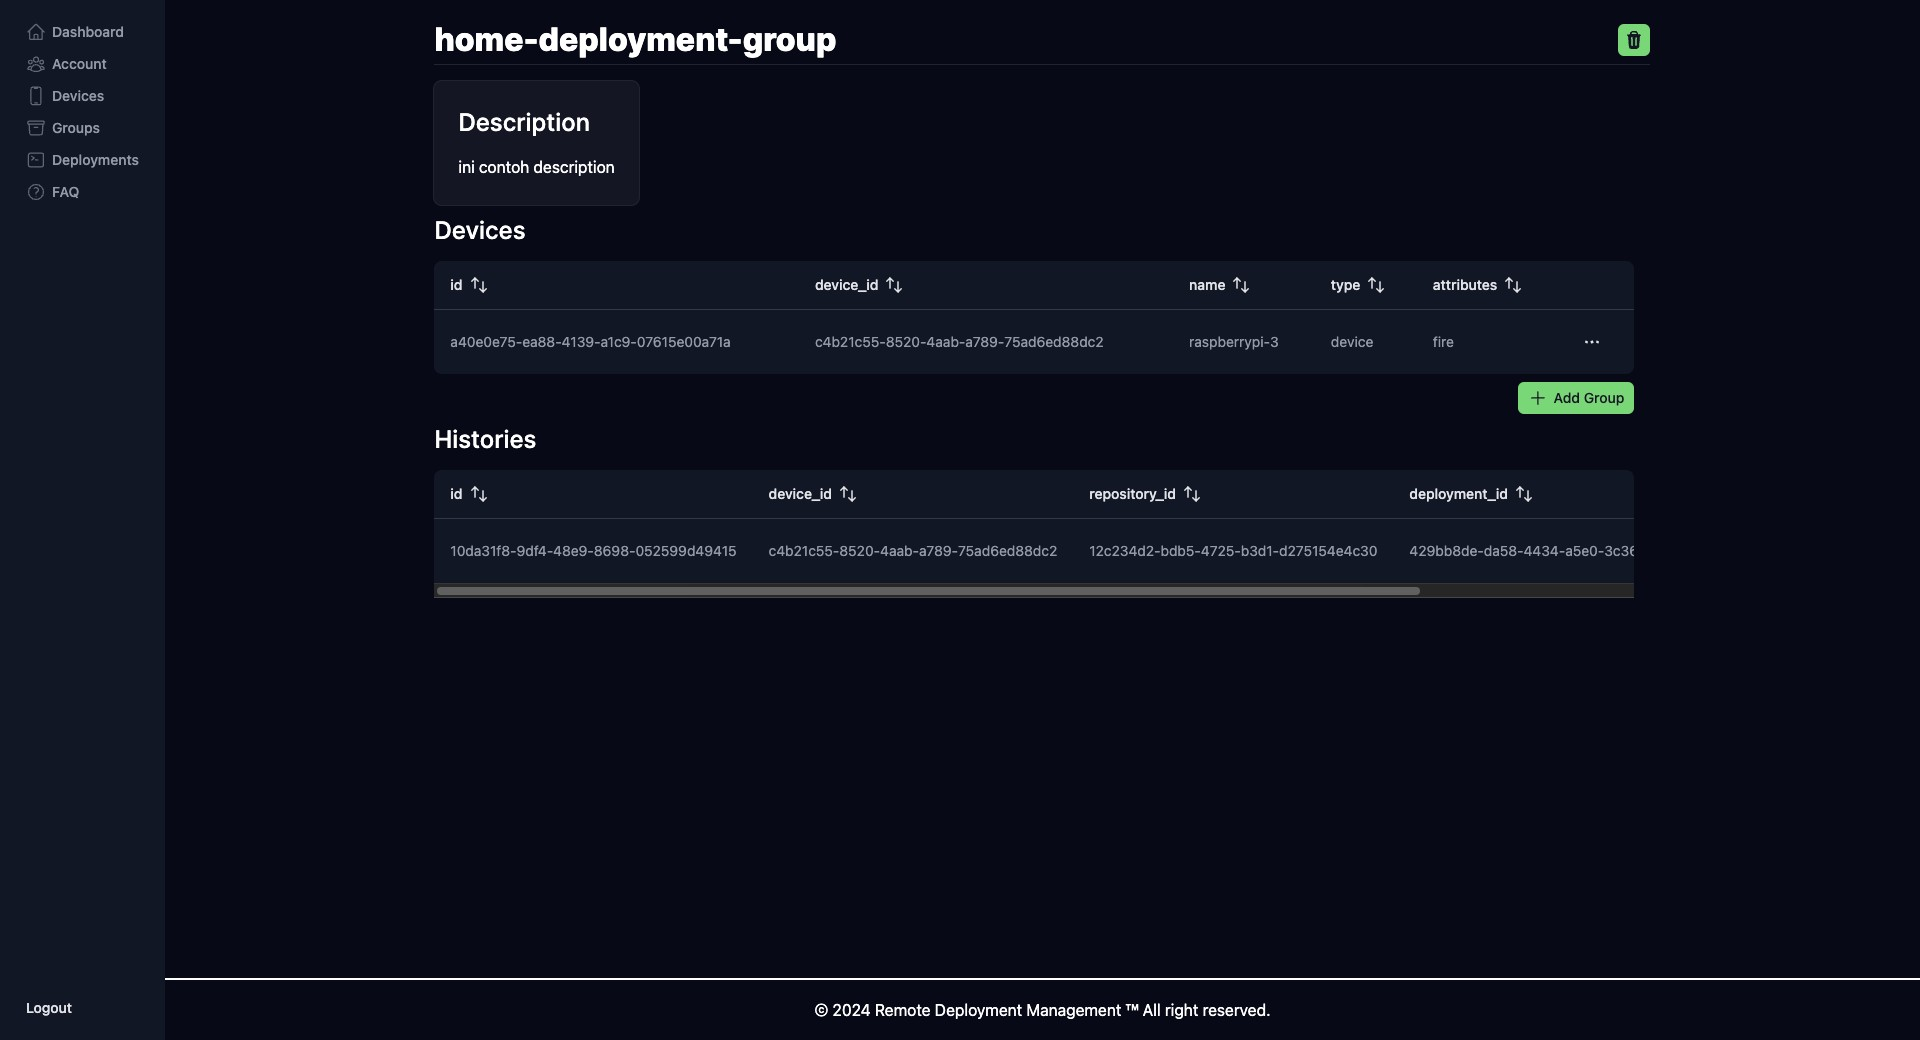
\includegraphics[width=1\textwidth]{resources/chapter-4/dashboard/groups-detail-page.jpg}
  \caption{Halaman \textit{groups detail}}
  \label{fig:halaman-groups-detail}
\end{figure}

halamann awkefljawkfejawkefaw

\begin{figure}
  \centering
  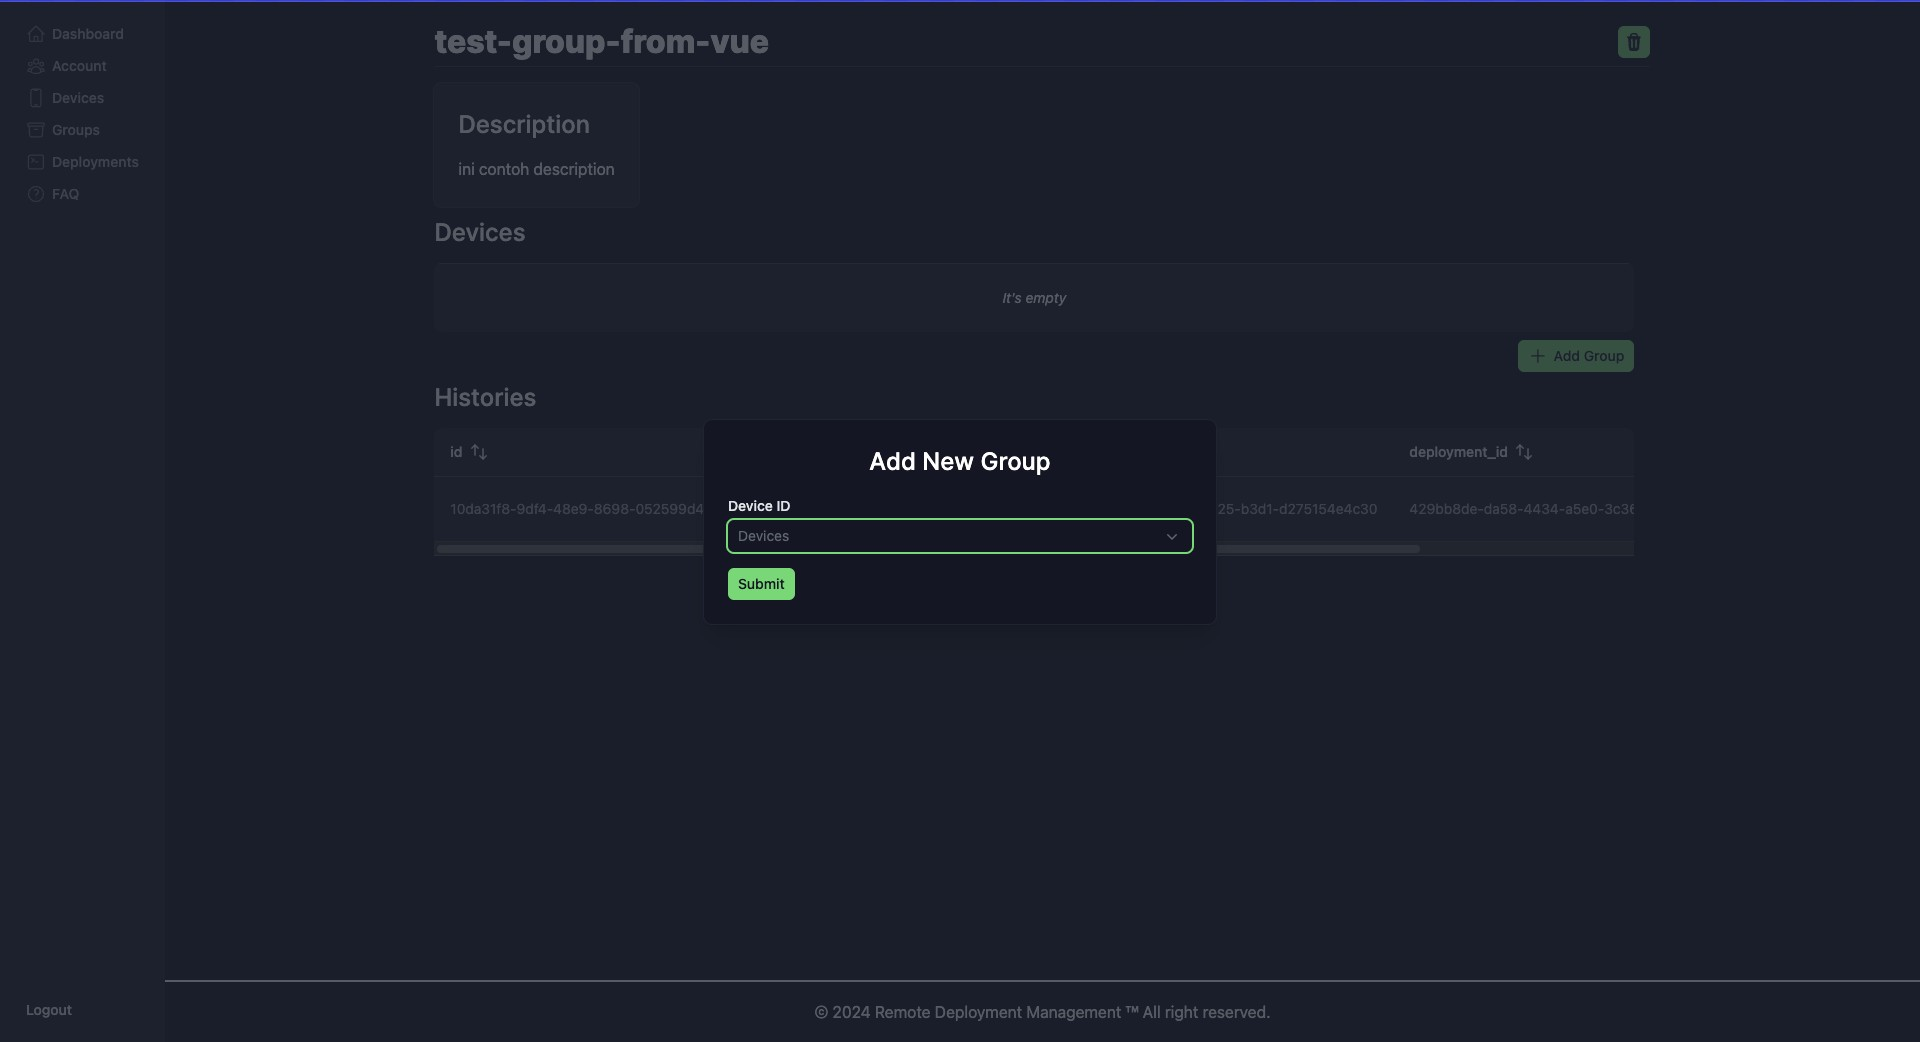
\includegraphics[width=1\textwidth]{resources/chapter-4/dashboard/groups-detail-add-device.jpg}
  \caption{Modal menambahkan group pada \textit{groups detail}}
  \label{fig:halaman-groups-detail-add-group}
\end{figure}

halamann awkefljawkfejawkefaw

\begin{figure}
  \centering
  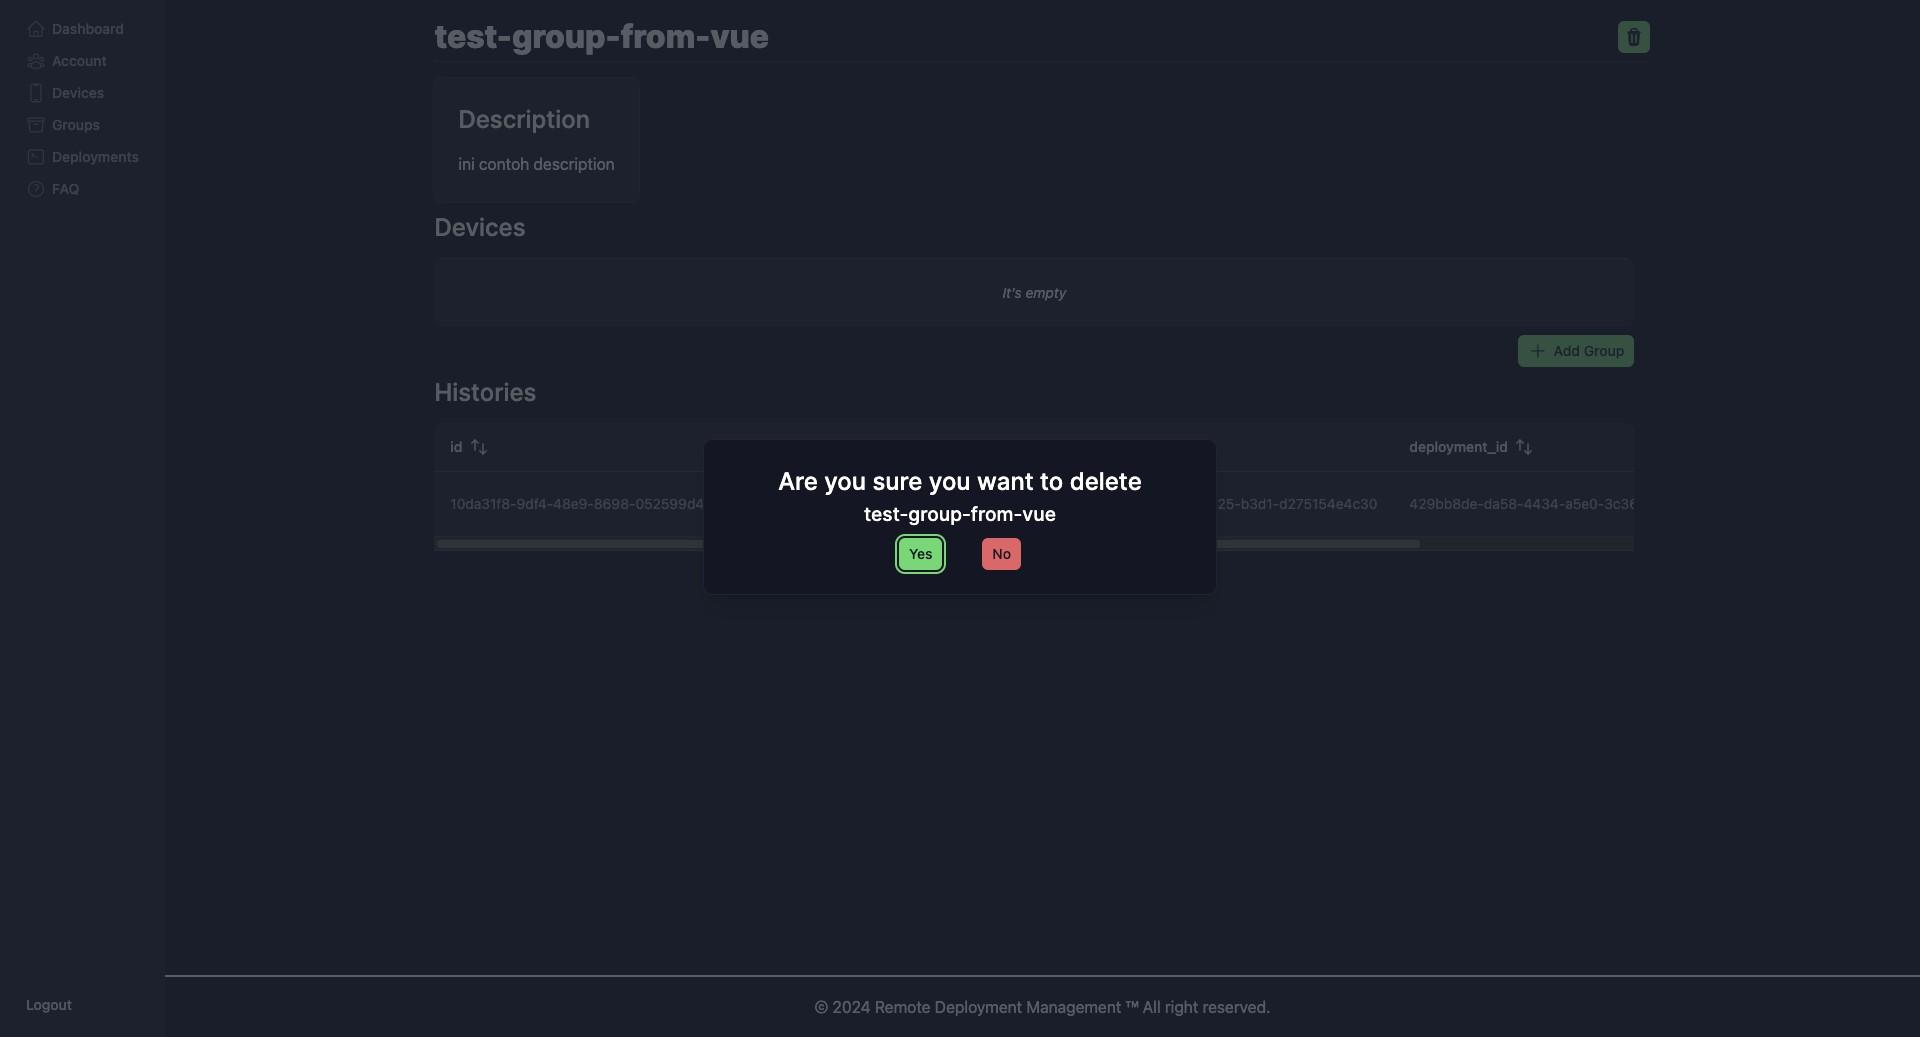
\includegraphics[width=1\textwidth]{resources/chapter-4/dashboard/groups-detail-delete.jpg}
  \caption{Modal menghapus groups pada halaman \textit{groups detail}}
  \label{fig:halaman-groups-detail-delete}
\end{figure}


\subsubsection{Halaman \textit{Deployment}}
penjelasan halaman deployment
\begin{figure}[h]
  \centering
  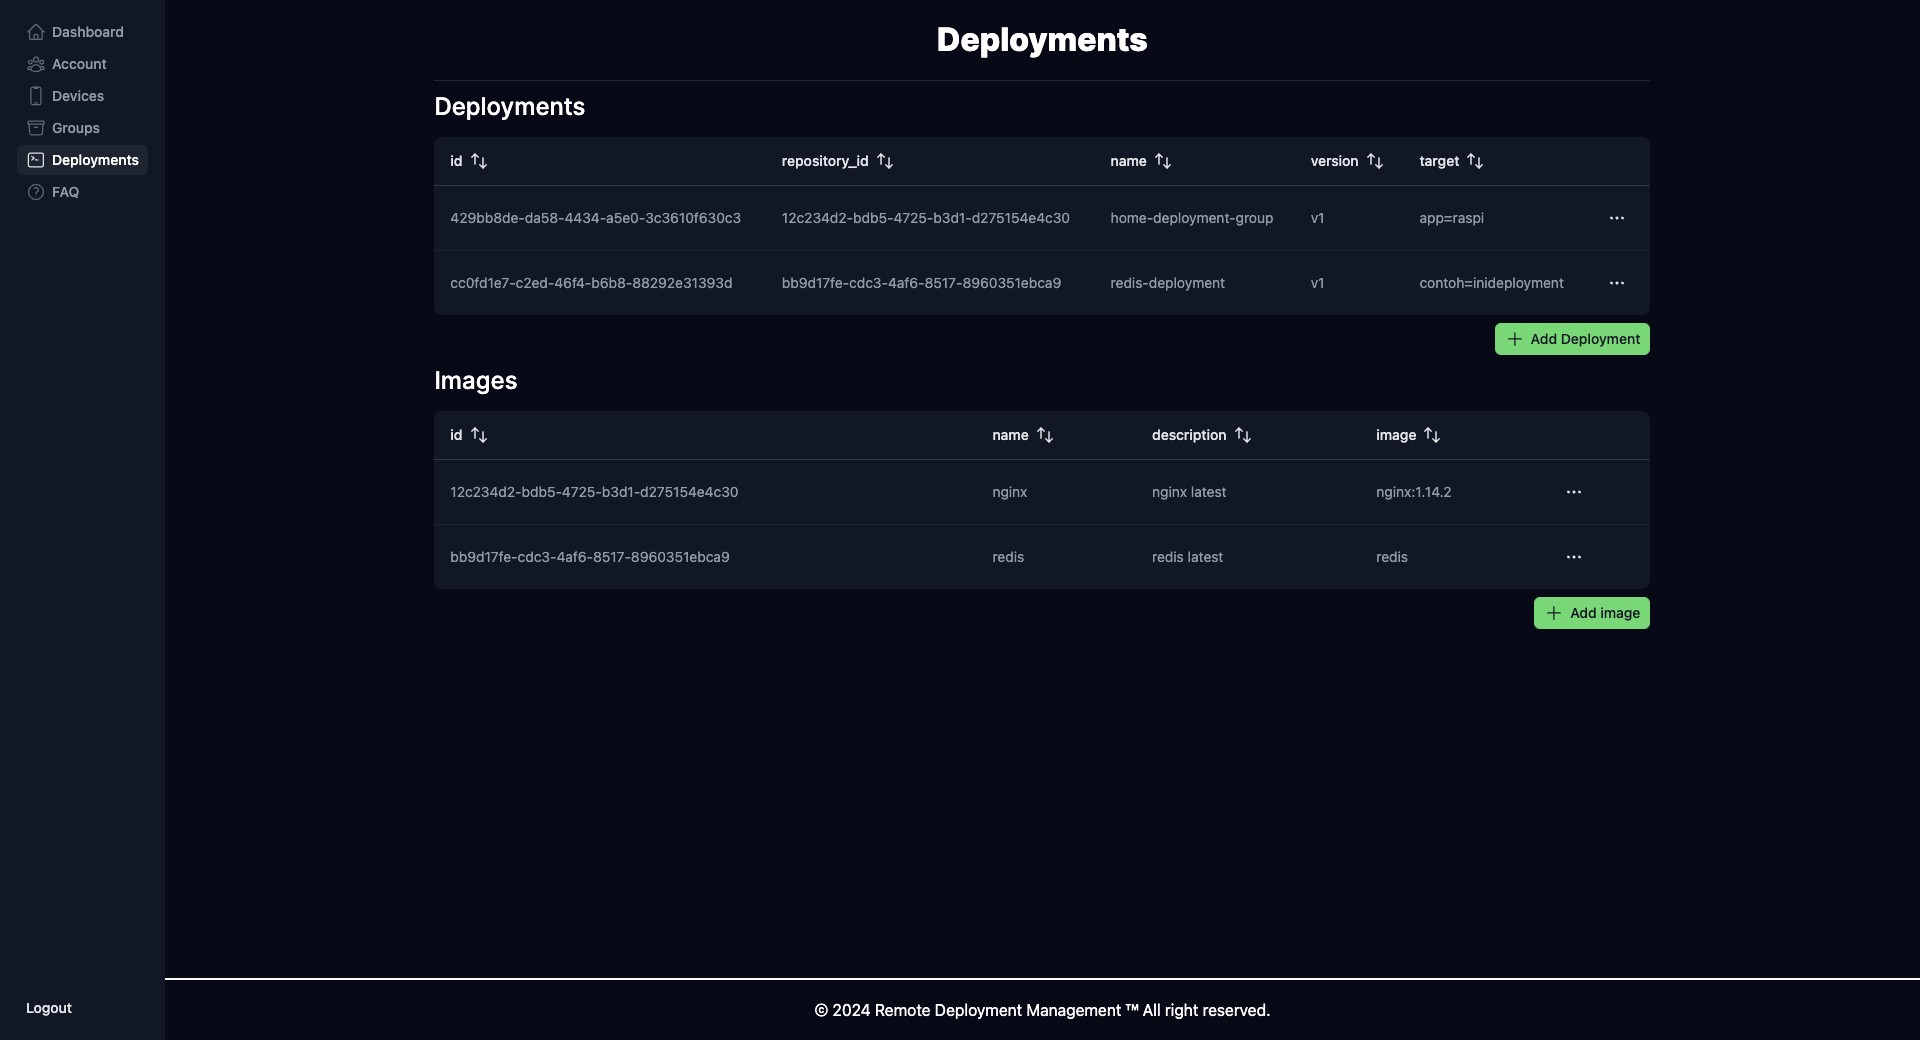
\includegraphics[width=1\textwidth]{resources/chapter-4/dashboard/deployment-page.jpg}
  \caption{Halaman \textit{deployment}}
  \label{fig:halaman-deployment}
\end{figure}

\begin{figure}[h]
  \centering
  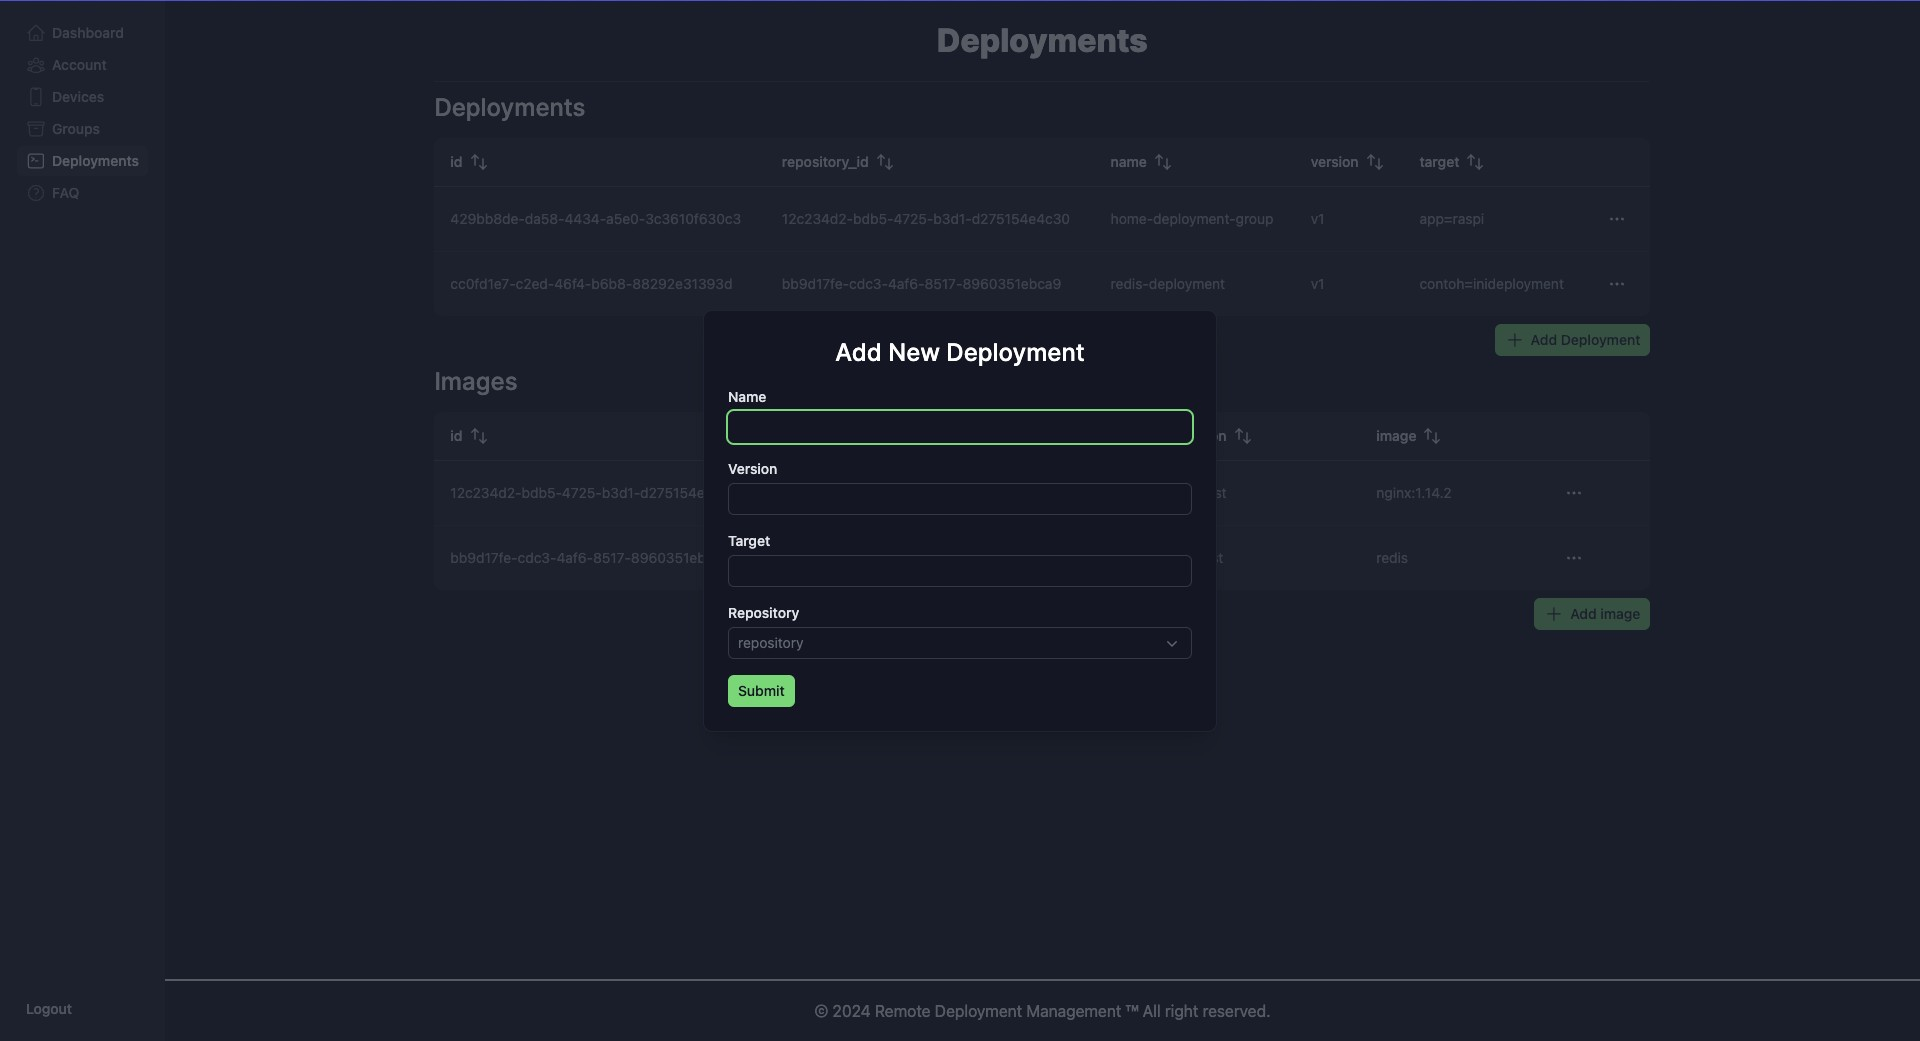
\includegraphics[width=1\textwidth]{resources/chapter-4/dashboard/deployment-page-add-deployment.jpg}
  \caption{Modal menambahkan \textit{deployment}}
  \label{fig:halaman-deployment-add-deployment}
\end{figure}

\begin{figure}[h]
  \centering
  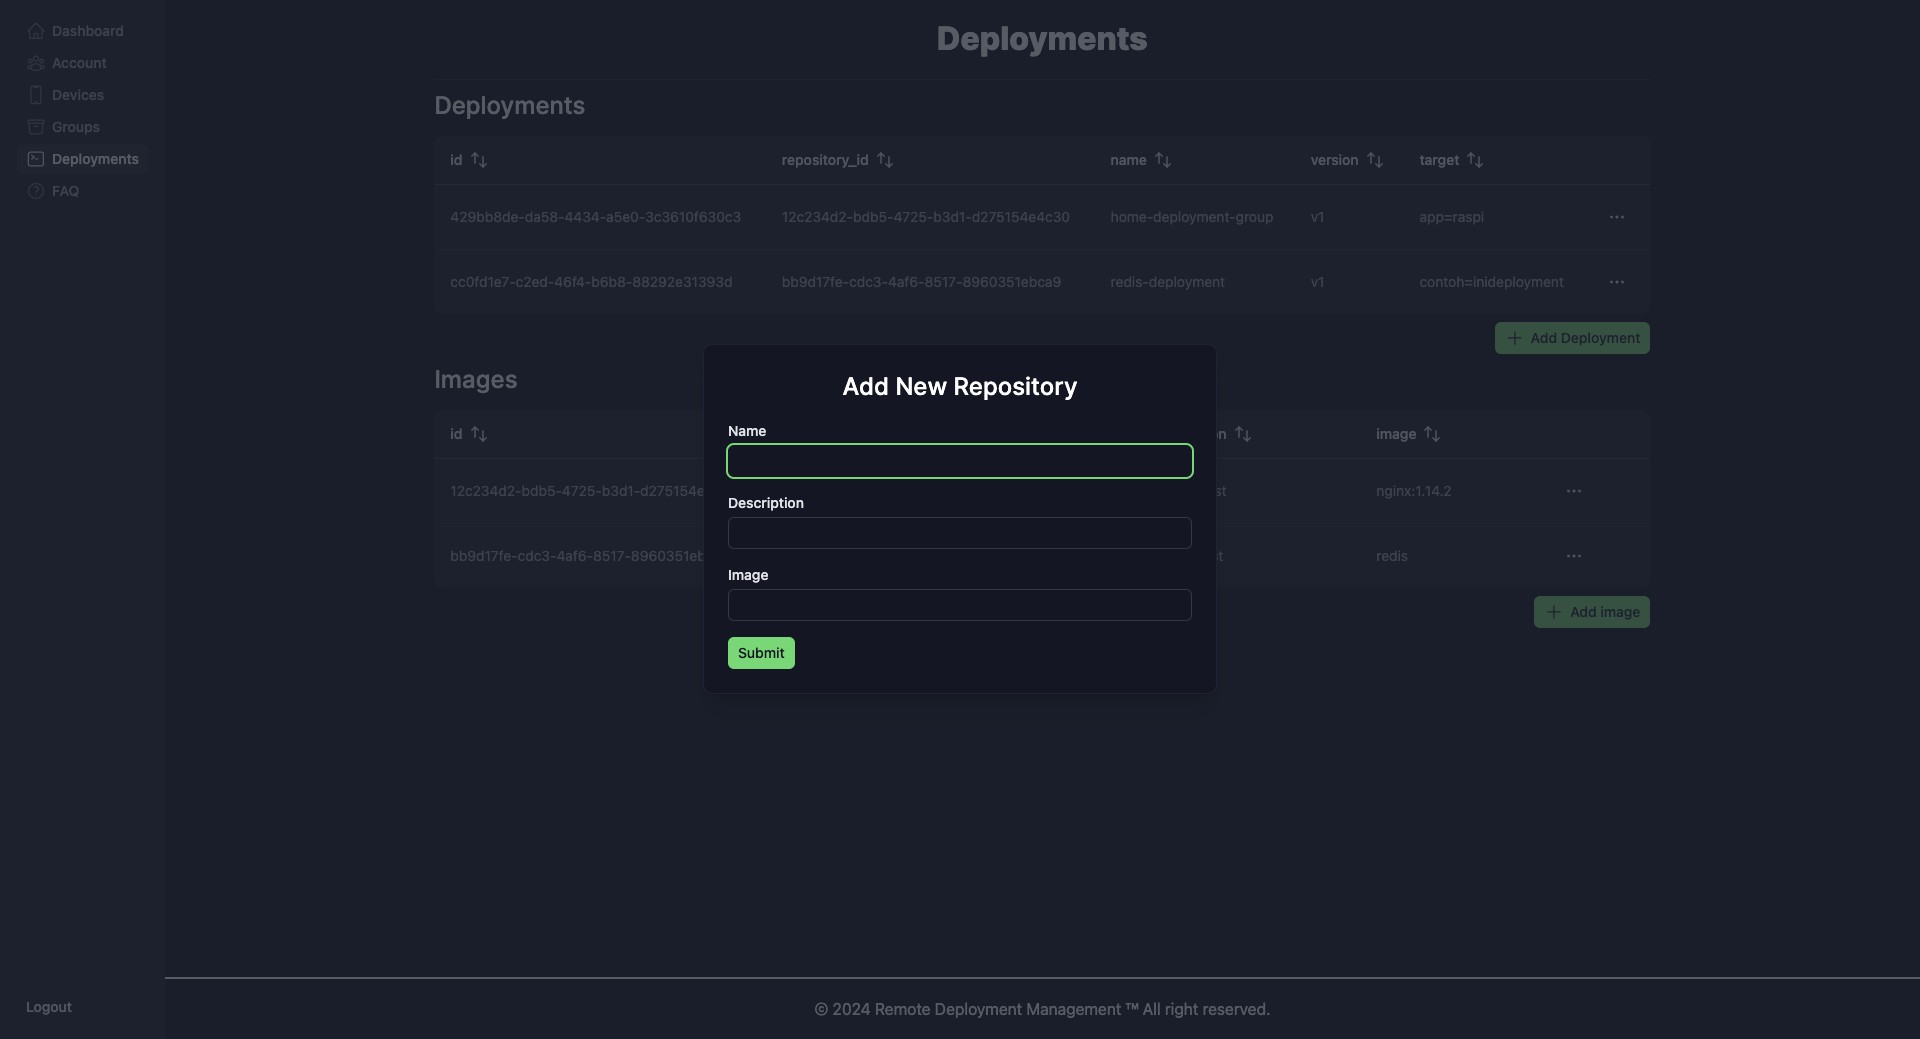
\includegraphics[width=1\textwidth]{resources/chapter-4/dashboard/deployment-page-add-repostory.jpg}
  \caption{Modal menambahkan \textit{image} pada halaman \textit{deployment}}
  \label{fig:halaman-deployment-add-repostory}
\end{figure}

\pagebreak

\subsubsection{Halaman \textit{deployments detail}}
penjelasan halaman deployments detail
\begin{figure}[h]
  \centering
  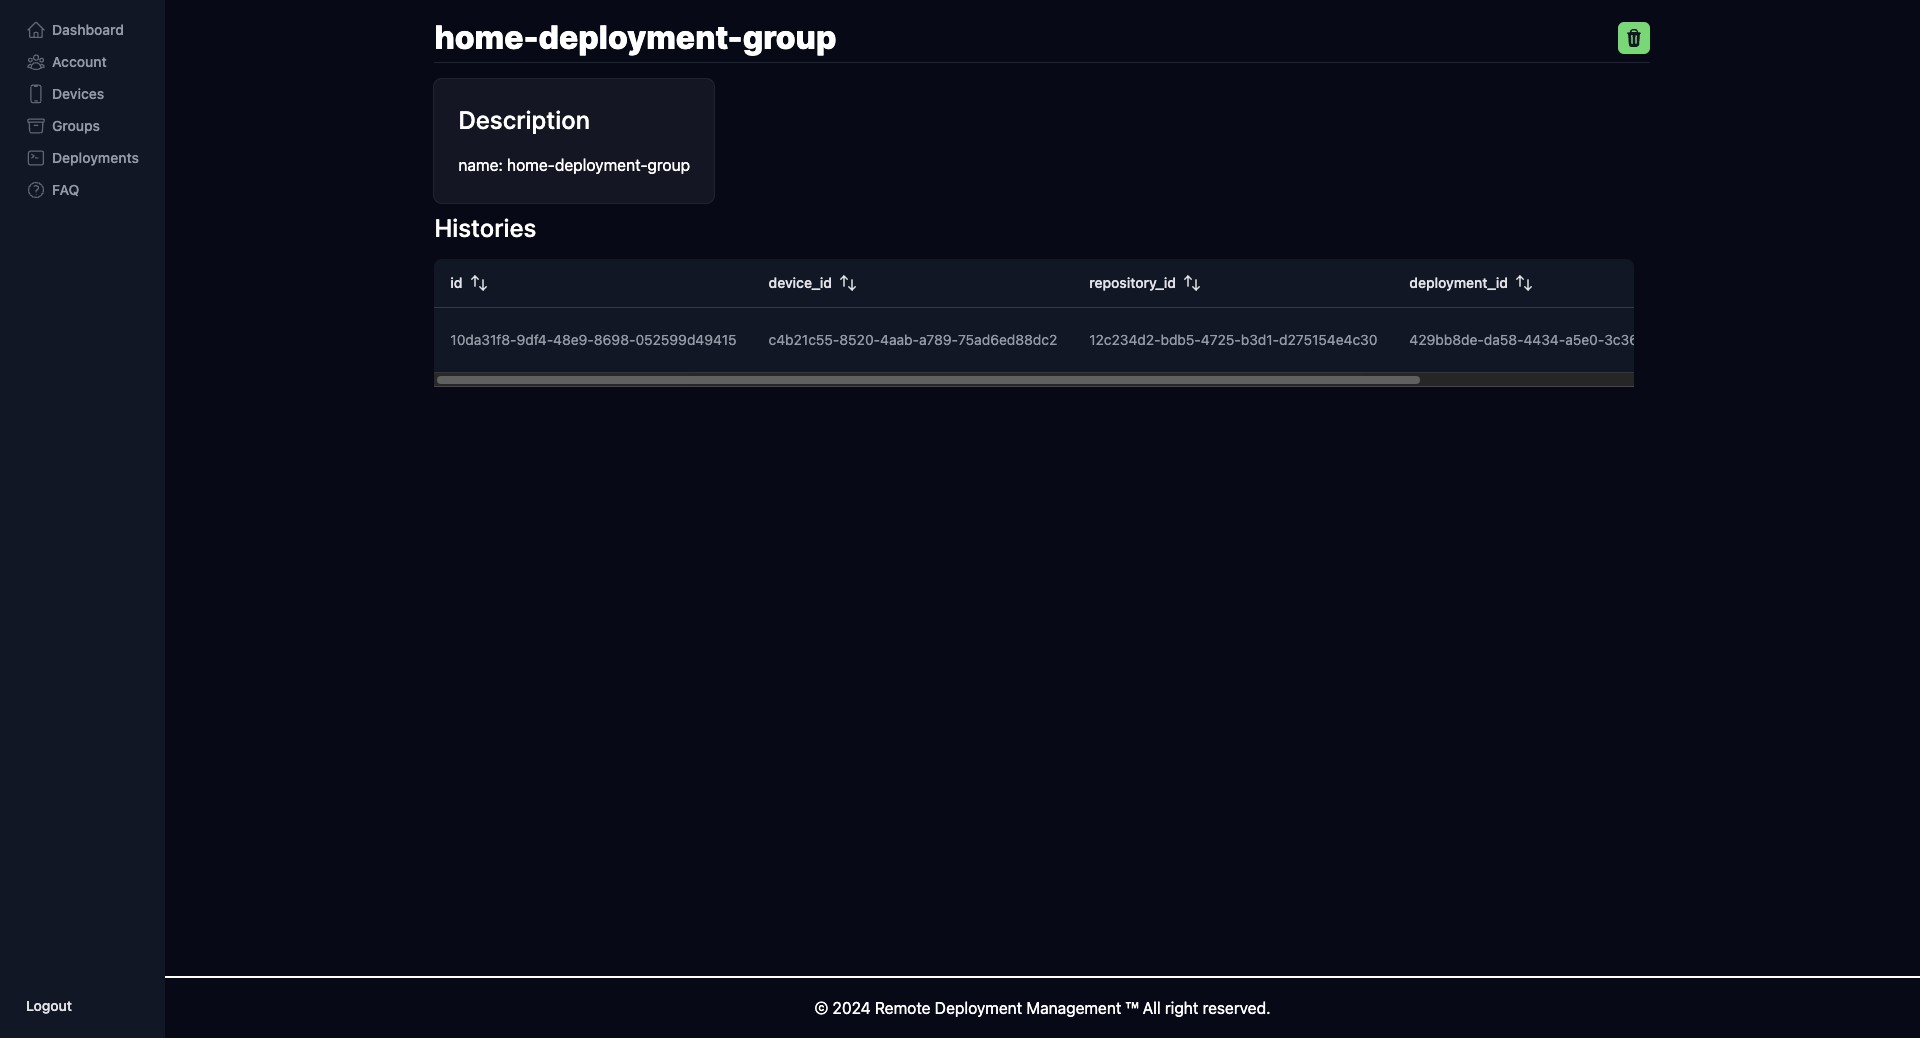
\includegraphics[width=1\textwidth]{resources/chapter-4/dashboard/deployment-detail-page.jpg}
  \caption{Halaman \textit{deployment detail}}
  \label{fig:halaman-deployment-detail}
\end{figure}

\begin{figure}[h]
  \centering
  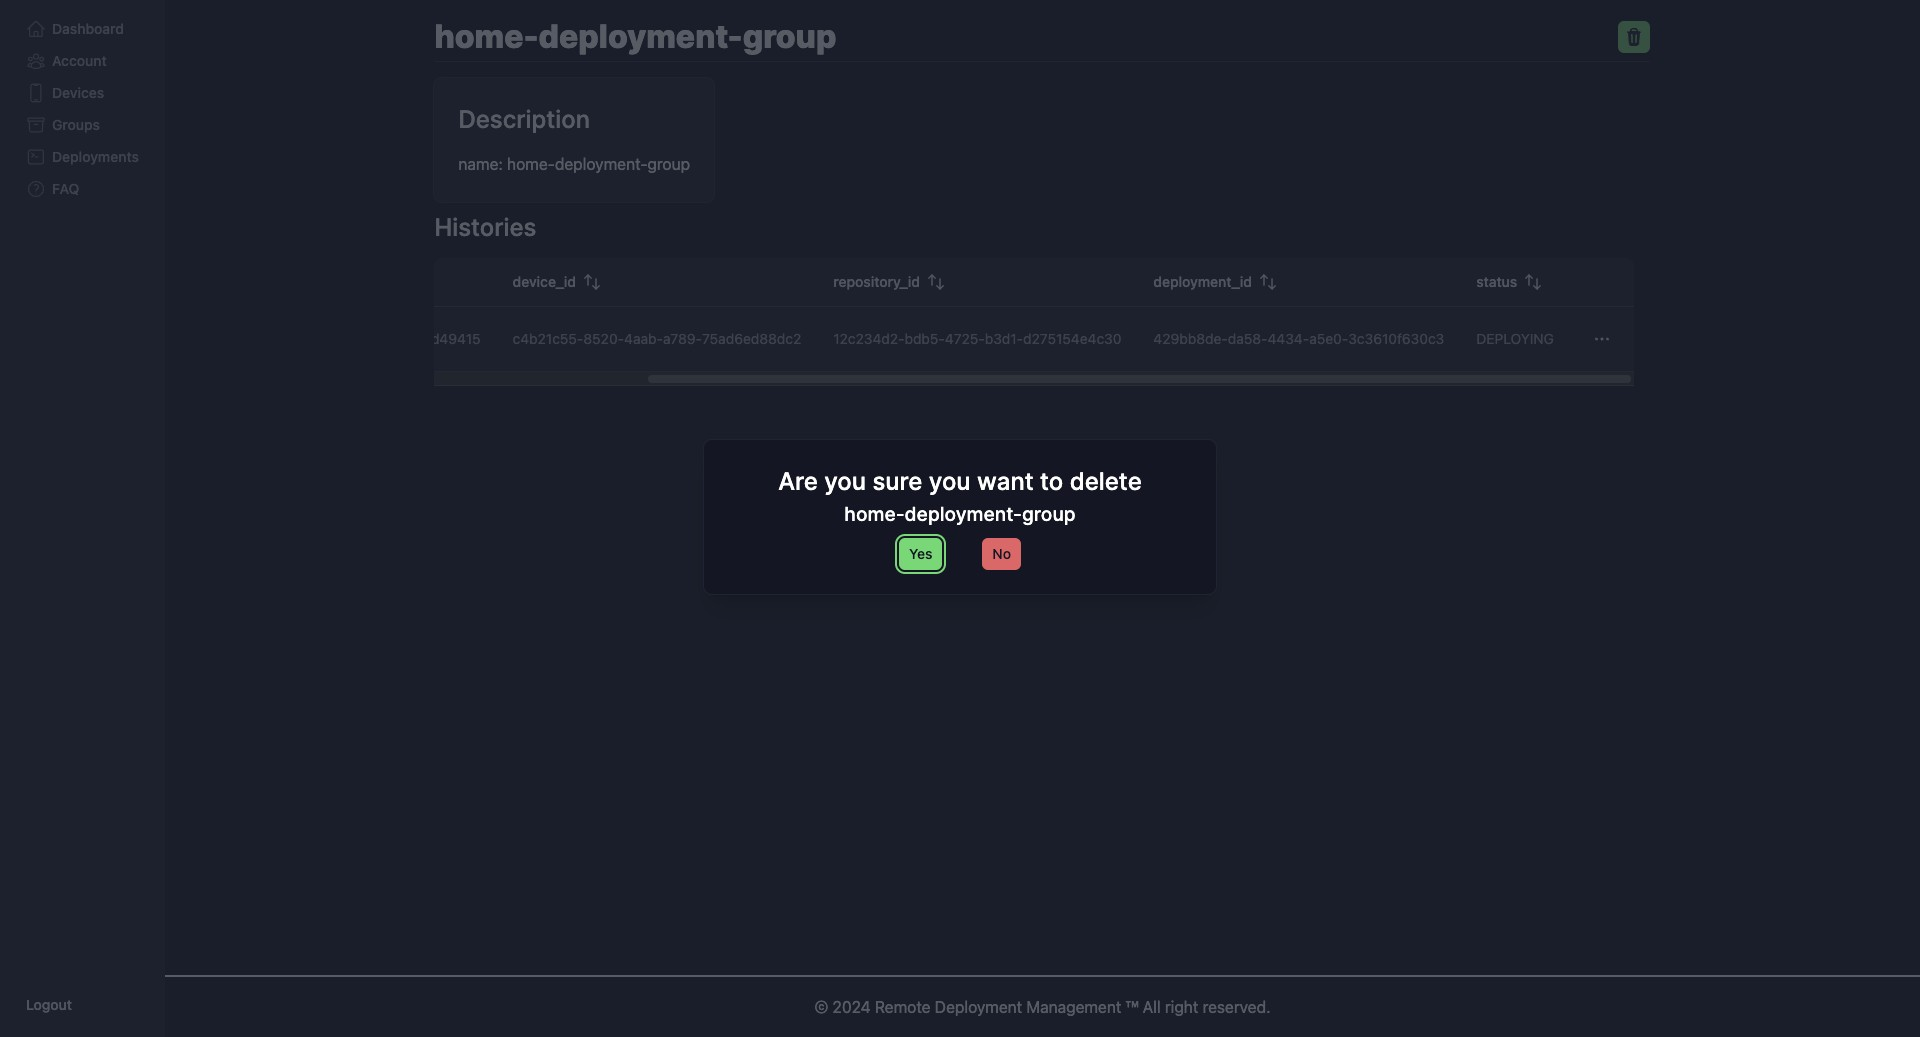
\includegraphics[width=1\textwidth]{resources/chapter-4/dashboard/deployment-detail-delete.jpg}
  \caption{Modal menghapus deployment pada halaman \textit{deployment detail}}
  \label{fig:halaman-deployment-detail-delete}
\end{figure}

\pagebreak

\subsubsection{Halaman \textit{history detail}}
Penjelasan halaman history detail

\subsubsection{Halaman \textit{FAQ}}
Penjelasan halaman faq

